\chapter{Symmetry and periodicity in photonics}
\label{h:periodic}

\begin{quote}
The mathematical sciences particularly exhibit order, symmetry, and limitation; and these are the greatest forms of the beautiful.

--- Aristotle
\end{quote}

\begin{quote}
Attaching significance to invariants is an effort to recognise what, because of its form or colour or meaning or otherwise, is important or significant in what is only trivial or ephemeral. A simple instance of failing in this is provided by the poll-man at Cambridge, who learnt perfectly how to factorise $a^2 - b^2$ but was floored because the examiner unkindly asked for the factors of $p^2 - q^2$.

--- H.W. Turnbull
\end{quote}

\chaptertoc

Systems which exhibit symmetry and periodicity are important in many areas of physics. One example are the periodic lattices in solid-state physics that can give rise to semiconductors. A similar phenomenon appears in photonics, as e.g. in so--called photonic crystals, which are artificial media where the refractive index has a periodicity on a scale of the order of the wavelength. This chapter introduces some concepts which are important for the study of these systems.

First, the scalar Helmholtz equation will be generalised to a vectorial equation which can also be used in the case of continuous index variations. We will interpret this as an eigenvalue problem, introduce the concept of a Hermitian operator and discuss some of the properties of such operators. This problem will also be cast in a variational framework, which will enable us to explain more of the physics of the eigenmodes.

Next, we will analyse how we can use symmetries to classify these eigenmodes, using the example of inversion symmetry. We will see that commuting operators play a key role when expressing symmetry. We will also discuss continuous translation symmetry, which is very relevant when studying e.g. waveguides. Finally, we will treat discrete translational symmetry or periodicity. This will allow us to talk about Bloch's theorem, Brillouin zones and band diagrams. 

To end, we will discuss time-reversal symmetry, as well as some applications of photonic crystals. We will briefly show how these periodic structures can be used to localise light in a cavity, or guide it along a waveguide.

\pagebreak



\sectionyoutubeugent{Helmholtz equation as an eigenvalue problem}{rKL8RE97lFw}

\begin{marginfigure}[-0.0cm]
  % credits: Wikipedia
  % url: https://en.wikipedia.org/wiki/Hermann_von_Helmholtz#/media/File:Hermann_von_Helmholtz.jpg
  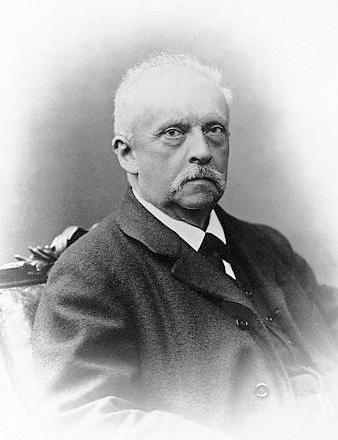
\includegraphics{helmholtz/figures/Hermann_von_Helmholtz}
  \caption{Hermann von Helmholtz (1821-1894)}
\end{marginfigure}

We will first derive the most general form of the vectorial Helmholtz equation which is also valid in the case of continuous refractive index variations. We start from

\begin{equation}
\nabla \times {\mathbf E({\mathbf r})} = - j \omega \mu {\mathbf H({\mathbf r})} \label{eq-maxwell-1}
\end{equation}
\begin{equation}   
\frac{1}{\varepsilon({\mathbf r})}\nabla \times {\mathbf H({\mathbf r})} = j \omega {\mathbf E({\mathbf r})} \label{eq-maxwell-2}
\end{equation}

\begin{cue}
Do a direct substitution of Eq.~\ref{eq-maxwell-2} into Eq.~\ref{eq-maxwell-1}.  
\end{cue}

Combining these equations results in

\begin{equation}
\fbox{$\displaystyle
\nabla \times \left[ \frac{1}{\varepsilon({\mathbf r})}\nabla \times {\mathbf H({\mathbf r})}  \right ] = \omega^2 \mu {\mathbf H({\mathbf r})} \label{eq-master}
$}
\end{equation} 

It is important not to yield to the temptation of bringing $\varepsilon({\mathbf r})$ outside of the $\nabla$--operator. This would be incorrect, because $\varepsilon$ is now no longer constant (although we assume that $\mu$ is constant since most 'normal' materials are non--magnetic).

Let's define the following linear differential operator:

\begin{equation}
\Theta \stackrel{def}{=} \nabla \times  \frac{1}{\varepsilon({\mathbf r})}\nabla \times
\end{equation} 

\begin{cue}
Use this operator to rewrite Eq.~\ref{eq-master}. What type of equation is this?   
\end{cue}

This operator takes the curl, divides by $\varepsilon({\mathbf r})$ and then takes the curl again. Using this notation, we can easily write Eq.~\ref{eq-master} as an eigenvalue problem:

\begin{equation}
\Theta {\mathbf H({\mathbf r})} = \omega^2 \mu {\mathbf H({\mathbf r})}
\end{equation} 

So, the eigenfunctions ${\mathbf H({\mathbf r})}$ of the $\Theta$--operator are field distributions that satisfy Maxwell's curl equations. The eigenvalues of these eigenfunctions are given by $\omega^2 \mu$. Note that in our current point-of-view $\omega$ is considered an unknown: for a given system with a certain index distribution, we are interested in finding the  $\omega$--values of the allowed solutions.

For physical reasons, we would obviously like these eigenvalues to be real and positive, as that would give rise to a real and positive value of the angular frequency $\omega$, provided that $\mu$ is real and positive.

To prove this, one of the concepts that we will need to use is that of \emph{Hermitian} operators.


\sectionugent{Hermitian operators}

\subsectionyoutube{Definition of Hermitian operators}{R34gCNeyeMU}

\noindent\marginnote{As should have become clear from earlier chapters, the choice of scalar product is somewhat arbitrary. Another choice would have been to omit the complex conjugate in the definition, but this would lose the link to a physical interpretation of the norm of a vector function as a real-valued energy.}To define what it means for an operator to be Hermitian, we first need to introduce a scalar product (also called inner product). Let's define this inner product between two vector functions ${\mathbf F({\mathbf r})}$ and ${\mathbf G({\mathbf r})}$ as

\begin{equation}
\fbox{$\displaystyle
\left\langle {\mathbf F}, {\mathbf G}\right\rangle = \iiint {\mathbf F^*({\mathbf r})} \cdot {\mathbf G({\mathbf r})} dV
$}
\end{equation} 

\begin{cue}
What can you say about $\left\langle {\mathbf G}, {\mathbf F}\right\rangle$? And what about $\left\langle {\mathbf F}, {\mathbf F}\right\rangle$? 
\end{cue}

From this simple definition, we immediately get that $\left\langle {\mathbf G}, {\mathbf F}\right\rangle = \left\langle {\mathbf F}, {\mathbf G}\right\rangle ^*$. We also see that $\left\langle {\mathbf F}, {\mathbf F}\right\rangle$ is always real and positive, even if ${\mathbf F}$ itself is complex.

Now, an operator $\Xi$ is said to be Hermitian if

\begin{equation}
\fbox{$\displaystyle
\left\langle {\mathbf F}, \Xi {\mathbf G}\right\rangle = \left\langle \Xi {\mathbf F}, {\mathbf G}\right\rangle
$}
\end{equation} 

This means that it doesn't matter which function is operated upon before taking the inner product. 

Clearly this is a special property which not all operators have, but it turns out that this is true for the $\Theta$ operator we defined above, in the context of the eigenproblem formulation of the Helmholtz equation. 

\pagebreak

\subsectionyoutube{$\Theta$ is a Hermitian operator}{VJGxvZBH1VM}

\begin{marginfigure}[0cm]
  % credits: Wikipedia
  % url: https://en.wikipedia.org/wiki/Charles_Hermite
  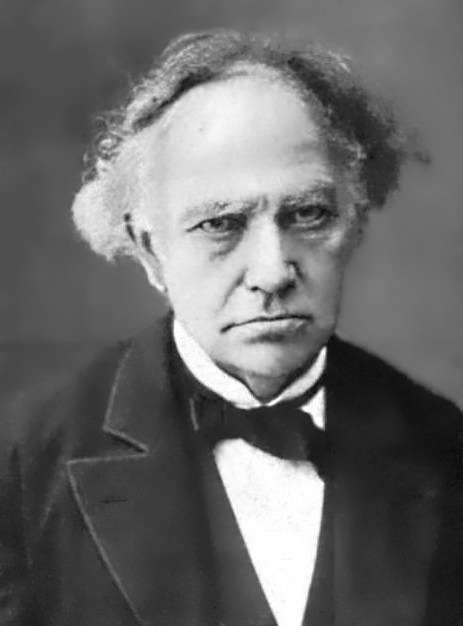
\includegraphics{hermite/figures/c_hermite}
  \caption{Charles Hermite (1822–1901)}
  \end{marginfigure}

Before showing that our operator $\Theta$ has this property, let's first derive an auxiliary result to help us manipulate the integrals involved in taking the scalar product. 

Let's start from

\begin{equation}
\nabla \cdot ({\mathbf a} \times {\mathbf b}) = {\mathbf b} \cdot ( \nabla \times {\mathbf a}) - {\mathbf a}  \cdot (\nabla \times {\mathbf b})
\end{equation} 

\begin{cue}
Integrate this over a volume and apply the divergence theorem.  
\end{cue}

we immediately get


\begin{equation}
\iiint {\mathbf a}  \cdot (\nabla \times {\mathbf b}) dV = \iiint {\mathbf b} \cdot ( \nabla \times {\mathbf a}) dV - \iiint \nabla \cdot ({\mathbf a} \times {\mathbf b}) dV 
\end{equation} 

With the divergence theorem, this can be written as

\begin{equation}
\iiint {\mathbf a}  \cdot (\nabla \times {\mathbf b}) dV = \iiint  ( \nabla \times {\mathbf a}) \cdot {\mathbf b} dV - \iint  {\mathbf a} \times {\mathbf b} \cdot d{\mathbf S} \label{eq-part-int}
\end{equation} 

This result allows us to move a curl operator from one factor of a scalar product to another factor, which will come in handy when we try to move our $\Theta$ operator in a similar way to prove hermiticity. 

\begin{cue}
Use the definition of  $\Theta$ in  $\left\langle {\mathbf F}, \Theta {\mathbf G}\right\rangle$ and apply the lemma we just derived.  
\end{cue}

Simply making use of definitions, we get

\begin{equation}
\left\langle {\mathbf F}, \Theta {\mathbf G}\right\rangle = \iiint {\mathbf F}^* \cdot\nabla \times \left[ \frac{1}{\varepsilon({\mathbf r})}\nabla \times {\mathbf G({\mathbf r})}  \right ] dV 
\end{equation} 

By applying our lemma Eq.~\ref{eq-part-int}, we get

\begin{equation}
\left\langle {\mathbf F}, \Theta {\mathbf G}\right\rangle = \iiint [ \nabla \times {\mathbf F}]^* \cdot \left[ \frac{1}{\varepsilon({\mathbf r})}\nabla \times {\mathbf G({\mathbf r})}  \right ] dV 
\label{eq-pos-omega}
\end{equation} 

Since $\nabla$ is real-valued, we were able to write $[ \nabla \times {\mathbf F}]^*$ instead of $\nabla \times {\mathbf F}^*$.

Also, the term related to the surface integral was dropped because in all practical cases, one of two things will be true. Either the fields at infinity will decay to zero, or the fields are periodic on the surface. In both cases, the surface term will vanish.

\begin{cue}
The second ingredient of $\Theta$ we need to bring over to operate on $ {\mathbf F}$ is  $\varepsilon$. Under which conditions are we allowed to do this?   
\end{cue}

If $\varepsilon$ is real (which will be the case for lossless media), we can write

\begin{equation}
\left\langle {\mathbf F}, \Theta {\mathbf G}\right\rangle = \iiint \left [\frac{1}{\varepsilon({\mathbf r})} \nabla \times {\mathbf F}\right]^* \cdot \left[ \nabla \times {\mathbf G({\mathbf r})}  \right ] dV 
\end{equation} 

\begin{cue}
Finally, bring the last curl operator over.
\end{cue}

Applying our lemma Eq.~\ref{eq-part-int} one more time, and again making use of the real-valued nature of $\nabla$, we get

\begin{equation}
\left\langle {\mathbf F}, \Theta {\mathbf G}\right\rangle = \iiint \left[ \nabla \times  \left [\frac{1}{\varepsilon({\mathbf r})} \nabla \times {\mathbf F}\right] \right ] ^* \cdot {\mathbf G({\mathbf r})}  dV  = \left\langle \Theta {\mathbf F}, {\mathbf G}\right\rangle 
\end{equation} 

This proves that our operator is indeed Hermitian.

\pagebreak

\begin{exer}
% difficulty: trivial
% ugent
% youtube: kamslD3uv5k
Are the following operators Hermitian?

a) $1$
  
b) $j$
  
c) $\nabla \times $

\begin{sol}
a) yes b) no c) yes
\end{sol}
\end{exer}

\begin{exer}
% difficulty: trivial
% ugent
% youtube: G7jRXZbzi2E
In this exercise, we will explore the relation between Hermitian operators and Hermitian matrices. As an operator working on a function, we take a matrix ${\mathbf A}$ which multiplies a column vector ${\mathbf x}$, i.e. the effect of the operator is given by ${\mathbf A} \cdot {\mathbf x}$. Let us define the scalar product between two column vectors as

$$\left\langle {\mathbf x},{\mathbf y} \right\rangle \stackrel{def}{=} {\mathbf x}^H \cdot {\mathbf y} = \sum{x_i^* y_i}$$

Now show that the operator defined by matrix multiplication by ${\mathbf A}$ is Hermitian if the matrix ${\mathbf A}$ is Hermitian, i.e. ${\mathbf A} = {\mathbf A}^H$.
\end{exer}


\begin{exer}
% difficulty: normal
% ugent
% youtube: gMN9QcJzojI
From Maxwell's curl equations, derive an eigenvalue problem for the electric field. Is the operator Hermitian?
\end{exer}

\pagebreak

\sectionugent{Properties of a Hermitian operator}
\label{week8}

\subsectionyoutube{The eigenvalues of a Hermitian operator are real}{7G3nAOaH3ds}

Let's return to our eigenvalue problem:

\begin{equation}
\Theta {\mathbf H} = \omega^2 \mu {\mathbf H}
\end{equation} 

\begin{cue}
Show that $\omega^2 \mu$ has to be real. Start by taking the inner product of this equation with ${\mathbf H({\mathbf r})}$, followed by taking the complex conjugate. Then apply what you know about the scalar product and about Hermitian operators.    
\end{cue}

Taking the inner product of this equation with ${\mathbf H({\mathbf r})}$, we get

\begin{equation}
\left\langle{\mathbf H} , \Theta {\mathbf H}\right\rangle  = \omega^2 \mu \left\langle {\mathbf H} , {\mathbf H}\right\rangle \label{eq-real-eigen-1}
\end{equation}

Now, taking the complex conjugate and using the fact that $\left\langle {\mathbf F}, {\mathbf F}\right\rangle$ is always real, we get

\begin{equation}
\left\langle{\mathbf H} , \Theta {\mathbf H}\right\rangle^*  = (\omega^2 \mu)^* \left\langle {\mathbf H} , {\mathbf H}\right\rangle 
\end{equation} 

Resist the temptation to say that $(\omega^2 \mu)^*= \omega^2 \mu $ for physical reasons, because that's exactly what we want to prove using only mathematical arguments.

For any operator $\left\langle {\mathbf G}, {\mathbf F}\right\rangle ^*  = \left\langle {\mathbf F}, {\mathbf G}\right\rangle$ such that

\begin{equation}
\left\langle \Theta {\mathbf H} , {\mathbf H} \right\rangle  = (\omega^2 \mu)^* \left\langle {\mathbf H} , {\mathbf H}\right\rangle 
\end{equation} 

But $\Theta$ is Hermitian, so we can write

\begin{equation}
\left\langle {\mathbf H} , \Theta {\mathbf H} \right\rangle  = (\omega^2 \mu)^* \left\langle {\mathbf H} , {\mathbf H}\right\rangle \label{eq-real-eigen-2}
\end{equation} 

Comparing Eq.~\ref{eq-real-eigen-1} and Eq.~\ref{eq-real-eigen-2}, we get that $(\omega^2 \mu)^* = \omega^2 \mu$, so \emph{the eigenvalues of a Hermitian operator are real}. If we now only consider lossless materials with real $\mu$, it immediately follows that $\omega^2$ is real.



\subsectionyoutube{The eigenvalues of $\Theta$ are positive}{hV9J5miSZgw}

Using a different argument, we can show that, at least for our operator $\Theta$, not only is the eigenvalue $\omega^2 \mu$ real, it is also positive, 

\begin{cue}
Set ${\mathbf F}={\mathbf G}={\mathbf H}$ in Eq.~\ref{eq-pos-omega} and use the fact that $\mathbf H$ is an eigenfunction of $\Theta$. Assume we are working with lossless dielectrics.
\end{cue}

Setting ${\mathbf F}={\mathbf G}={\mathbf H}$ in Eq.~\ref{eq-pos-omega}, we get

\begin{equation}
\left\langle {\mathbf H}, \Theta {\mathbf H}\right\rangle = \iiint \frac{1}{\varepsilon({\mathbf r})} \left | \nabla \times {\mathbf H({\mathbf r})} \right |^2  dV 
\label{eq-rot-H-bis}
\end{equation} 

With Eq.~\ref{eq-real-eigen-1} this becomes

\begin{equation}
\omega^2 \mu \left\langle {\mathbf H} , {\mathbf H}\right\rangle = \iiint \frac{1}{\varepsilon({\mathbf r})} \left | \nabla \times {\mathbf H({\mathbf r})} \right |^2  dV \label{eq-omega-pos}
\end{equation} 

For lossless dielectrics $\varepsilon$ is real and positive. Since now all terms in Eq.~\ref{eq-omega-pos} are positive, $\omega^2$ must be positive too. So, we can pick the positive square root, leading to a positive $\omega$ and a physical interpretation.

Let's stress again that the fact that the eigenvalues are positive here, is due to the special form of our operator. It is \emph{not} a general property of Hermitian operators.



\pagebreak

\subsectionyoutube{The eigenfunctions of a Hermitian operator are orthogonal}{UlFuOt7wCrQ}

Consider two eigenfunctions (modes) ${\mathbf H}_1$ and ${\mathbf H}_2$ with frequencies $\omega_1$ and $\omega_2$.

\begin{cue}
Using the fact that these are eigenmodes of $\Theta$, calculate $\left\langle {\mathbf H}_1 , \Theta {\mathbf H}_2\right\rangle$ and $\left\langle \Theta {\mathbf H}_1 , {\mathbf H}_2\right\rangle$. 
\end{cue}
  
Because ${\mathbf H}_1$ and ${\mathbf H}_2$ are eigenfunctions of $\Theta$ we can write

\begin{equation}
 \left\langle {\mathbf H}_1 , \Theta {\mathbf H}_2\right\rangle = \omega_2^2 \mu \left\langle {\mathbf H}_1 , {\mathbf H}_2\right\rangle 
\label{eq-ortho-1}
\end{equation}

and

\begin{equation}
 \left\langle \Theta {\mathbf H}_1 , {\mathbf H}_2\right\rangle = \omega_1^2 \mu \left\langle {\mathbf H}_1 , {\mathbf H}_2\right\rangle
\label{eq-ortho-2}
\end{equation}

\begin{cue}
Subtract these two equations. When are the modes ${\mathbf H}_1$ and ${\mathbf H}_2$ orthogonal? 
\end{cue}

Because $\Theta$ is hermitian, the left--hand sides of Eq.~\ref{eq-ortho-1} and Eq.~\ref{eq-ortho-2} are equal, so we get

\begin{equation}
(\omega_2^2 - \omega_1^2) \left\langle {\mathbf H}_1 , {\mathbf H}_2\right\rangle = 0
\end{equation} 

If $\omega_1 \ne \omega_2$, we have $\left\langle {\mathbf H}_1 , {\mathbf H}_2\right\rangle = 0$ and we can conclude that ${\mathbf H}_1$ and ${\mathbf H}_2$ are orthogonal modes.

\noindent\marginnote{Solutions which only differ by a proportionality constant are not considered to be degenerate, but rather, they are considered to be the ``same'' mode.}In the special case where two different modes have the same frequency $\omega_1 = \omega_2$, we call them \textbf{degenerate modes}, which are not necessarily orthogonal. However, since $\Theta$ is a linear operator, any linear combination of these degenerate eigenmodes will also be an eigenmode with the same frequency. This means that we can always choose to work with linear combinations that are orthogonal. These combinations can be obtained by e.g. a Gram--Schmidt orthogonalisation procedure.

\pagebreak

\begin{exer}
  % difficulty: trivial
  % ugent
  % youtube: UnBQdfE-0S0
  
  Which of the following statements are true for a Hermitian eigenvalue problem?

  a) All eigenvalues are real.

  b) All eigenvalues are positive.

  c) All eigenfunctions are orthogonal.

  d) Two eigenfunctions $\mathbf H$ and $\alpha\mathbf H$, with $\alpha$ a scalar, are considered to be degenerate.
  
  \begin{sol}
    a) true b) false c) false (you can construct an orthogonal set, but they are in general not orthogonal, e.g. when you have degeneracy.) d) false
  \end{sol}

\end{exer}

\pagebreak

\sectionugent{Variational interpretation of the Helmholtz eigenvalue problem}
\label{sec-sym-var}

\subsectionyoutube{A variational form of the Helmholtz eigenvalue problem}{aotPwYLJ2aA}

In order to get some general feeling for the nature of the modes and derive some more of their properties, it is useful to look at a variational form:

\begin{equation}
J \stackrel{def}{=} \frac{\left\langle {\mathbf H} , \Theta {\mathbf H}\right\rangle}{\left\langle {\mathbf H} , {\mathbf H}\right\rangle} \label{eq-variational}
\end{equation}  

We will show that any function ${\mathbf H}$ for which $J$ is stationary (i.e. $\delta J=0$) will satisfy our eigenvalue problem.

We can calculate the first variation of $J$ directly from Eq.~\ref{eq-variational}. However, it turns out that the calculation is a bit easier if we first rewrite Eq.~\ref{eq-variational} as

\begin{equation}
\left\langle {\mathbf H},{\mathbf H} \right\rangle J = \left\langle {\mathbf H},\Theta {\mathbf H} \right\rangle \label{eq-variational-1}
\end{equation} 

\begin{cue}
'Perturb' this equation, i.e. replace ${\mathbf H}$ by ${\mathbf H} + \delta {\mathbf H}$ and $J$ by a corresponding $J+ \delta J$. Then, subtract the original from the perturbed equation, and neglect higher-order terms.  
\end{cue}

Replacing ${\mathbf H}$ by ${\mathbf H} + \delta {\mathbf H}$ and $J$ by $J+ \delta J$, we get:

\begin{align}
\left\langle {\mathbf H + \delta {\mathbf H}},{\mathbf H}+\delta {\mathbf H} \right\rangle J + \left\langle {\mathbf H}+\delta {\mathbf H},{\mathbf H+\delta {\mathbf H}} \right\rangle \delta  J \nonumber  \\
  = \left\langle {\mathbf H}+\delta {\mathbf H},\Theta {\mathbf H} + \Theta \delta {\mathbf H} \right\rangle
\label{eq-variational-2}
\end{align} 

Subtracting Eq.~\ref{eq-variational-1} from Eq.~\ref{eq-variational-2} and neglecting higher-order variations gives


\begin{equation}
\left\langle \delta {\mathbf H},{\mathbf H} \right\rangle J + \left\langle {\mathbf H},\delta {\mathbf H} \right\rangle J + \left\langle {\mathbf H}, {\mathbf H} \right\rangle \delta J = \left\langle {\mathbf H},\Theta \delta {\mathbf H} \right\rangle + \left\langle \delta {\mathbf H},\Theta {\mathbf H} \right\rangle \label{eq-variational-3}
\end{equation} 


\pagebreak

\begin{exer}
% difficulty: trivial
% youtube: ODn9Gr2xdVY
Show that we can transform Eq.~\ref{eq-variational-3} to

$$\delta J = \frac {\left\langle \delta {\mathbf H} , {\mathbf G} \right\rangle + \left\langle {\mathbf G} , \delta {\mathbf H} \right\rangle}{2}$$

with

$${\mathbf G} \stackrel{def}{=} \frac{2}{\left\langle {\mathbf H} , {\mathbf H}\right\rangle } \left[ \Theta {\mathbf H} - \frac{\left\langle {\mathbf H} , \Theta {\mathbf H}\right\rangle}{\left\langle {\mathbf H} , {\mathbf H}\right\rangle} {\mathbf H} \right]  $$
\end{exer}

\begin{cue}
Use this expression to find the Euler-Lagrange equation for this variational form.  
\end{cue}

Now, if $\delta J$ needs to be zero for all possible ${\delta \mathbf H}$, this means that ${\mathbf G}$ should be equal to zero, or

\begin{equation}
\Theta {\mathbf H} = \frac{\left\langle {\mathbf H} , \Theta {\mathbf H}\right\rangle}{\left\langle {\mathbf H} , {\mathbf H}\right\rangle} {\mathbf H} \label{eq-variational-4}
\end{equation} 

Bearing in mind that the quotient on the right-hand side is just a number, Eq.~\ref{eq-variational-4} can only be fulfilled if ${\mathbf H}$ is indeed an eigenvector of $\Theta$. Incidentally, we have also proven that its eigenvalue is $J$.


\pagebreak
\subsectionyoutube{Physical insights from the variational form of the Helmholtz eigenvalue problem}{f398ScBbwfM}

Having survived the gory mathematical details of verifying that Eq.~\ref{eq-variational} is indeed the variational expression of our eigenvalue problem, it's time to do something useful with it and derive a physical heuristic for the modes in our system.

\begin{cue}
Evaluate $J$ if ${\mathbf H}$ is a solution to the eigenvalue problem. What does the result mean for the frequency of the modes?  
\end{cue}
  
First, in case ${\mathbf H}$ is a solution to the eigenvalue problem, $J$ becomes

\begin{equation}
J =  \frac{\left\langle {\mathbf H} , \Theta {\mathbf H}\right\rangle}{\left\langle {\mathbf H} , {\mathbf H}\right\rangle} = \frac{\left\langle {\mathbf H} , \omega^2 \mu {\mathbf H}\right\rangle}{\left\langle {\mathbf H} , {\mathbf H}\right\rangle} = \omega^2 \mu
\end{equation}

Apart from verifying again that in its extremal points $J$ is the eigenvalue, this shows that solutions ${\mathbf H}$ which have low values of $J$ will tend to have a low frequency $\omega$. So, \textbf{lower-order solutions will have lower frequencies/energies} in comparison to higher-order solutions.

\begin{cue}
Use Eq.~\ref{eq-rot-H-bis} to write $J$ as an expression containing a volume integral of $ \nabla \times {\mathbf H({\mathbf r})}$ in the numerator.   
\end{cue}

Second, using Eq.~\ref{eq-rot-H-bis}, we can write the functional as

\begin{align}
J =& \frac{1}{\left\langle {\mathbf H} , {\mathbf H}\right\rangle}  \iiint \frac{1}{\varepsilon({\mathbf r})} \left | \nabla \times {\mathbf H({\mathbf r})} \right |^2  dV  \label{eq-variational-HH}
\end{align} 

\pagebreak

\begin{exer}
  % difficulty: normal
  % youtube: Tw5EOfN30mY
When ${\mathbf H}$ is a solution to the eigenvalue problem, transform Eq.~\ref{eq-variational-HH} into the following form, which contains only the electric field:
$$J=\frac{\iiint \left | \nabla \times {\mathbf E({\mathbf r})} \right |^2  dV} {\iiint \epsilon \left | {\mathbf E({\mathbf r})} \right |^2  dV} $$
\label{ex-eigenvalue-e}
\end{exer}

\begin{cue}
Looking separately at the numerator and the denominator of this expression, what properties does ${\mathbf E}$ need to have in order to minimise $J$?   
\end{cue}

From this equation, we can see that $J$ is minimised if \textbf{the electric field ${\mathbf E}$ is concentrated in regions where the refractive index is high}. So, to minimise $J$, a mode will try to concentrate its field in regions of high dielectric, while remaining orthogonal to the modes below it in frequency. With this heuristic we can e.g. explain why it is that dielectric waveguides do indeed work: the field likes to be concentrated in regions where the refractive index is high. Also, because of the link between $J$ and $\omega$, concentrating a mode in regions of high refractive index (thus lowering $J$) will tend to lower its frequency.

As a third point, the same equation also suggests that to minimise $J$, it is advantageous to keep spatial variations in the field as low as possible, so as to keep  $\left| \nabla \times {\mathbf E({\mathbf r})} \right |$ small. This explains why \textbf{the fundamental mode has much slower spatial variations than the higher-order modes}.

Finally, remember that all modes are orthogonal to each other, so e.g. the first-order mode 'finds' the most energetically favourable solution in the subspace perpendicular to the fundamental mode.

We will use these heuristics in a later section to explain the peculiar behaviour of certain periodic structures.

\pagebreak

\begin{exer}
  % difficulty: normal
  % youtube: pE88UxlZaUA
Show that, if you have two Hermitian operators $A$ and $B$, the generalised eigenvalue problem $A {\mathbf H} = \lambda B {\mathbf H}$ is the Euler-Lagrange equation of the following variational expression: \\

$$J = \frac{\left\langle {\mathbf H} , A {\mathbf H}\right\rangle}{\left\langle {\mathbf H} , B {\mathbf H}\right\rangle}$$

What is $\lambda$? (Note that ${\mathbf H}$ is a general vector function, not per se the magnetic field.)

\end{exer}

\begin{exer}
  % difficulty: normal
  % youtube: GQGkpIUZUso
Derive a generalised eigenvalue problem for $\mathbf E$. Under what conditions is it Hermitian, i.e. are the two operators $A$ and $B$ involved in the generalised eigenvalue problem Hermitian? Note that it should be a true generalised eigenvalue problem, i.e. with $B$ not equal to the identity operator.

\end{exer}

\begin{exer}
  % difficulty: trivial
  % youtube: Iu1NIrRO7u4
Show based on the previous two exercises that minimising the following variational expression is equivalent to solving Maxwell's equations: \\

$$J=\frac{\iiint \left| \nabla \times {\mathbf E ({\mathbf r})} \right| ^2  dV} {\iiint \epsilon \left| {\mathbf E ({\mathbf r})} \right| ^2  dV}$$

(This is the same result as in Ex.~\ref{ex-eigenvalue-e}, but the derivation there assumed that we were starting from an existing solution $\mathbf H$. The approach here is much more general.)

\end{exer}


\pagebreak


\sectionyoutubeugent{Eigensolutions in structures with inversion symmetry}{qrPcB0DVElI}

In this section, we start discussing how symmetries can be helpful to classify the solutions of Eq.~\ref{eq-master}, without actually needing to solve the eigenproblem explicitly. We'll do this using the example of inversion symmetry.

\begin{cue}
What other symmetries do you know? How would you define a symmetry mathematically?  
\end{cue}

In general, a symmetry is any change of coordinates which leaves the form of Eq.~\ref{eq-master} intact. E.g., suppose you have a circular cavity, then any rotation of the coordinate system around the central axis will result in an identical situation. Other examples of symmetries are mirror symmetry, translational symmetry, etc. 

\begin{marginfigure}
\centering
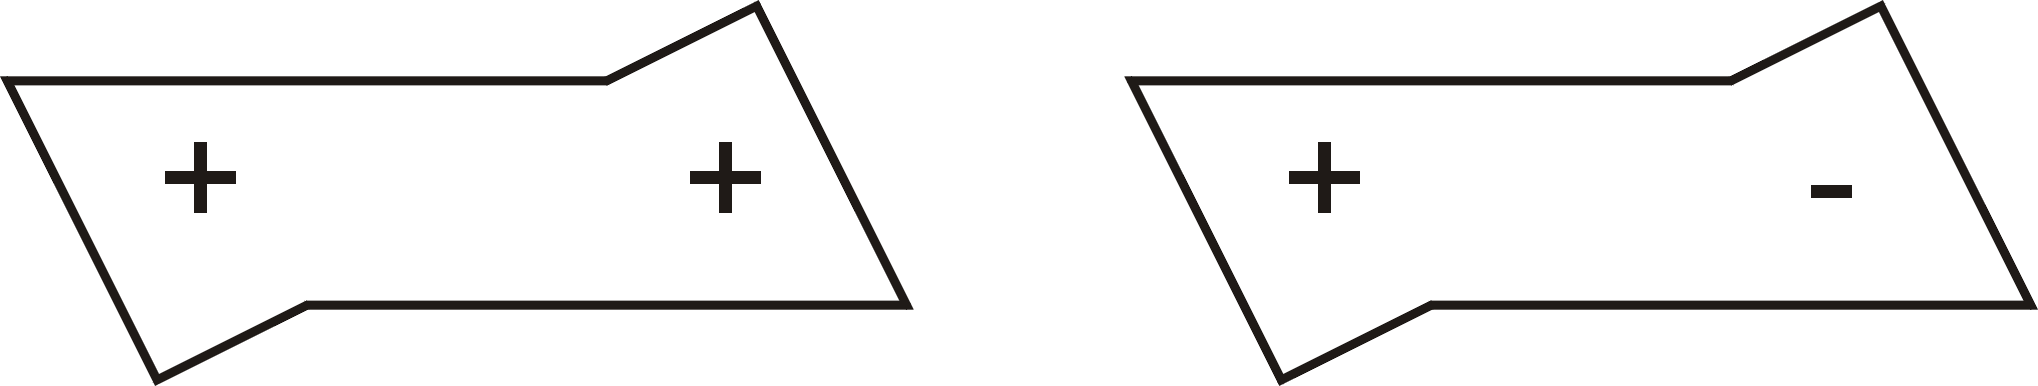
\includegraphics{symmetry/figures/symmcav}
\caption{A 2D metal cavity with inversion symmetry. On the left, an even mode with ${\mathbf H}({\mathbf r}) = {\mathbf H}(-{\mathbf r})$, on the right an odd mode with ${\mathbf H}({\mathbf r})=-{\mathbf H}(-{\mathbf r})$.}
\label{fig-symmcav}
\end{marginfigure}

To illustrate what symmetries can teach us about the existence of certain families of solutions, we will focus on the example of inversion symmetry. Let's look at the structure from Fig.~\ref{fig-symmcav}, a creatively shaped metal cavity that is inversion symmetric around its centre $\mathbf{r}=0$.

\begin{cue}
Under what coordinate transformation is Fig.~\ref{fig-symmcav} invariant?   
\end{cue}

This structure is invariant under the coordinate change ${\mathbf r}' = -{\mathbf r}$.

Suppose we want to find the modes (i.e. the solutions to Maxwell's equations for a certain frequency $\omega$) of the cavity from Fig.~\ref{fig-symmcav}. Solving Maxwell's equations for such a cavity will not be possible analytically, but we know that the structure possesses symmetry: by inverting it about its centre, you end up with the same shape.

\begin{cue}
How would you formulate this in terms of the field pattern ${\mathbf H({\mathbf r})}$ of a solution to Maxwell's equations?    
\end{cue}

If somehow we find that a particular pattern ${\mathbf H({\mathbf r})}$ is a mode of the cavity with frequency $\omega$, then ${\mathbf H(-{\mathbf r})}$ must also be a mode with frequency $\omega$, since the cavity cannot tell ${\mathbf r}$ from ${-\mathbf{r}}$.

\begin{cue}
In case there is no degeneracy, what does that mean for the relation between ${\mathbf H({\mathbf r})}$ and ${\mathbf H({\mathbf{-r}})}$?    
\end{cue}

Suppose ${\mathbf H({\mathbf r})}$ is not degenerate, so that it is the only mode at frequency $\omega$. Then, since ${\mathbf H(-{\mathbf{r}})}$ is also a mode with frequency $\omega$, it must really be the same mode! This means that it must be a straightforward multiple of ${\mathbf H({\mathbf r})}$:

\begin{equation}
{\mathbf H(-{\mathbf{r}})} = \alpha {\mathbf H({\mathbf r})}
\end{equation} 

\begin{cue}
Repeat the inversion and figure out the possible values for $\alpha$.    
\end{cue}

To determine $\alpha$, we can invert the system twice, meaning that we return to the original function ${\mathbf H({\mathbf r})}$ and pick up another factor $\alpha$ in the process. So

\begin{equation}
{\mathbf H(-(-{\mathbf{r}}))} = \alpha {\mathbf H(-{\mathbf r})} = \alpha^2 {\mathbf H({\mathbf r})}
\end{equation} 

\noindent\marginnote{This is not true for degenerate modes. But, although we do not prove it here, we can always form new modes which \emph{are} even or odd, by taking appropriate linear combinations of degenerate modes.}This means that $\alpha$ is either 1 or -1. So, a given nondegenerate mode must be one of two types: either it is invariant under inversion, ${\mathbf H(-{\mathbf r})} = {\mathbf H({\mathbf r})}$, and we call it \textbf{even}, or it becomes its own opposite under inversion, ${\mathbf H(-{\mathbf r})} = - {\mathbf H({\mathbf r})}$ and we call it \textbf{odd}.

\vspace{1cm}

\begin{exer}
  % difficulty: trivial
  % ugent
  % youtube: S9JhZb0LSJw
  For a system with inversion symmetry, and in case you have degenerate modes, is it still the case that if ${\mathbf H({\mathbf r})}$ is a mode of the cavity, then ${\mathbf H(-{\mathbf r})}$ is always a mode as well?  

\begin{sol}
Yes
\end{sol}
\end{exer}

\pagebreak

\sectionyoutubeugent{Commutators and symmetry}{}

We have classified the modes based on how they respond to one of the cavity's symmetry operations. Let's place this on a slightly more mathematical footing, which can also be generalised more easily. 

\noindent\marginnote{To generalise this, just use any operator that expresses a symmetry of our system.}Suppose $O_I$ is an operator that inverts vector fields ${\mathbf H({\mathbf r})}$. Now, what is the mathematical expression that our system $\Theta$ has inversion symmetry? Since inversion is a symmetry of our system, it does not matter whether we do one of the following two things:

\begin{itemize}
\item
 We operate with $\Theta$ on a certain function.
\item
\noindent\marginnote{We do have to go back to the original coordinate system, otherwise we'd be comparing apples to oranges.}We first invert the coordinates, then operate with $\Theta$ and then change the coordinates back.
\end{itemize}

Graphically, this corresponds to the diagram in Fig.~\ref{fig-commutator}.

\begin{marginfigure}[1.0cm]
 \includegraphics{symmetry/figures/commutator}
 \caption{Using operators to express that a system has symmetry.}
 \label{fig-commutator} 
\end{marginfigure}

\begin{cue}
How would you translate the observations above in a formula?
\end{cue}

Expressing this mathematically, we get:

\begin{equation}
  \Theta = O_I^{-1} \Theta O_I
  \label{eq-operator-symmetry}
\end{equation} 

When looking at the right-hand side of the equation, note that operators are being evaluated from right to left, because by definition the argument of an operator is always placed to its right.

Eq.~\ref{eq-operator-symmetry} can trivially be rearranged as

$$O_I \Theta - \Theta O_I = 0$$

\begin{exer}
  % difficulty: trivial
  % youtube: _ReuEQ6QMUs
Draw a diagram similar to Fig.~\ref{fig-commutator} that expresses this relation.
\end{exer}

\noindent\marginnote{The name is well-chosen: if the commutator is zero, the two operations commute, i.e. their order does not matter.}Just like in quantum mechanics, we can define the \textbf{commutator} $[A,B]$ of two operators $A$ and $B$ as

\begin{equation}
 \fbox{$\displaystyle
   [A,B] \stackrel{def}{=} AB - BA
 $}
\end{equation} 

So, we have shown that \textbf{our system is symmetric under inversion only if the inversion operator commutes with $\Theta$}.

Note that the commutator is itself an operator. 

\begin{cue}
Operate with this commutator on a solution ${\mathbf H({\mathbf r})}$, making use of the fact that this is an eigenmode of $\Theta$. Can you use the result to identify a new eigenmode for $\Theta$? 
\end{cue}

If we now operate with this commutator on any mode ${\mathbf H({\mathbf r})}$ of the system, we get

\begin{equation}
[O_I, \Theta] {\mathbf H}= O_I \left(\Theta {\mathbf H} \right) - \Theta \left(O_I {\mathbf H} \right) = 0
\end{equation} 

This means that

\begin{equation}
\Theta \left(O_I {\mathbf H} \right) = O_I \left( \Theta {\mathbf H} \right) = O_I \left( \omega^2 \mu {\mathbf H}\right)
\end{equation} 

Or

\begin{equation}
\Theta \left(O_I {\mathbf H} \right) =  \omega^2 \mu \left(O_I {\mathbf H}\right)
\end{equation} 

This is nothing other than saying that if ${\mathbf H}$ is an eigenmode with frequency $\omega$, then $O_I {\mathbf H}$ is also an eigenmode with the same frequency.

\begin{cue}
Assuming no degeneracy, what does this mean?
\end{cue}

In the absence of degeneracy, there can only be one mode per frequency, so ${\mathbf H}$ and $O_I {\mathbf H}$ can only differ by a multiplicative factor.

\begin{cue}
Formulate this mathematically. What kind of an equation is this?
\end{cue}

This means $O_I {\mathbf H} = \alpha {\mathbf H}$. This is actually an eigenvalue equation for $O_I$, and we already know from the previous section that its eigenvalues $\alpha$ are 1 and -1. 

Tracing back, we see that we started from a function ${\mathbf H}$ that was an eigenvector of $\Theta$ and ended up by showing that the same ${\mathbf H}$ was also an eigenvector of $O_I$ (at least in the absence of degeneracy). 

But what if there is degeneracy in the system? In that case, two modes might have the same frequency, even though they are not related by a simple multiplier. Again, although we won't show it here, in that case it will still be possible to construct different linear combinations of these degenerate modes to make new modes which themselves are even or odd, or - more generally - are eigenfunctions of the symmetry operator.

So, \textbf{if two operators commute, it is possible to construct joint eigenfunctions ${\mathbf H}$ of both operators}, i.e. functions ${\mathbf H}$ that are solutions of both eigenproblems $\Theta {\mathbf H} = \omega^2 \mu {\mathbf H}$ and $O_I {\mathbf H} = \alpha {\mathbf H}$.

This is very convenient, as eigenvectors and eigenvalues for simple symmetry operators can be easily determined, whereas those for $\Theta$ cannot. So, without solving the eigenproblem for $\Theta$ explicitly, we can still make useful statements about the existence of different classes of solutions, based on the properties of the symmetry operation.

\begin{exer}
  % difficulty: trivial
  % youtube: H0vg0kd0aJc
  If you have a function which is an eigenfunction of two operators, show that the commutator of these operators operating on that eigenfunction yields zero.
\end{exer}

\begin{exer}
  % difficulty: normal
  % youtube: mTzBgy8nql8
What is the commutator of $x$ and $d/dx$?  
\end{exer}

\begin{exer}
  % difficulty: normal
  % youtube: -kdWUB_dYnM
Given two linear operators $\mathbf A$ and $\mathbf B$, under which circumstances is

$$\left ( {\mathbf A} + {\mathbf B} \right ) ^2 =  {\mathbf A}^2 + 2 {\mathbf A}{\mathbf B}  + {\mathbf B}^2$$

For which exercise from chapter \ref{h:hermite} is this relevant?
\begin{sol}
When $\mathbf A$ and $\mathbf B$ commute.
\end{sol}
\end{exer}

\begin{exer}
  % difficulty: normal
  % youtube: OzDu5ECj1dA
True or false: if a system described by an operator $\Theta$ has a symmetry described by an operator $O$, then all eigenfunctions of $\Theta$ and $O$ are common.
  \begin{sol}
    False
\end{sol}  
\end{exer}

\pagebreak

\sectionyoutubeugent{Eigensolutions in structures with continuous translation symmetry}{}

One way of saying that our system is unchanged by a translation over a displacement ${\mathbf d}$ is

\begin{equation}
\varepsilon ({\mathbf r} + {\mathbf d}) =  \varepsilon ({\mathbf r})
\end{equation} 

We can also define a translation operator $T_{\mathbf d}$:

\begin{equation}
T_{\mathbf d} \varepsilon ({\mathbf r}) \stackrel{def}{=} \varepsilon ({\mathbf r} + {\mathbf d})
\end{equation} 

Just like before, saying that our system in invariant under that operator amounts to $[\Theta, T_{\mathbf d}] = 0$.

A system with \emph{continuous} translation symmetry in the $z$--direction is invariant for all $T_{\mathbf d}$ in that direction. So, $\Theta$ must commute with all the translation operators over a distance ${\mathbf d} = d {\mathbf 1}_z$. In order not to make the notation too heavy, we will limit ourselves here to scalar fields which only vary in the $z$--direction.

\begin{cue}
  Using what you know about eigenfunctions of operators that commute, what can you say? Be careful to make your statements general enough so that they hold for translations over all ${d}$.
\end{cue}

We know that we can construct modes of $\Theta$ that are eigenfunctions of these translation operators $T_d$ as well:

\begin{equation}
T_d H(z) = H(z + d) = \lambda(d) H(z)
\end{equation} 

This has to be true for all possible $d$, but the eigenvalues $\lambda$ can be different for each $d$, which is why we write them as $\lambda(d)$. 

\begin{cue}
Compare a single translation over $d+d'$ to a sequence of two translations, first over $d$, then over $d'$. What does this teach you about the dependence of $\lambda$ on $d$?
\end{cue}

Geometrically it is obvious that a translation over $d$ followed by a translation over $d'$ is equivalent to a single translation over $d+d'$:

\begin{equation}
T_{d+d'}H(z) = T_{d'}T_{d}H(z)
\end{equation} 

This means that

\begin{equation}
\lambda(d + d')=\lambda(d')\lambda(d)
\end{equation} 

\begin{cue}
What is the most general function that converts sums to products like that?
\end{cue}

\noindent\marginnote[2cm]{The factor $-j$ is there to satisfy conventions.}A function which behaves that way is the exponential. However, $e^d$ is not general enough. Actually, there has to exist a number $k_z$ such that

\begin{equation}
\lambda(d) = e^{-j k_z d}
\end{equation} 

So, we can use this number $k_z$ as a label to classify the different modes, just like we classified modes with inversion symmetry based on whether their eigenvalue for $O_I$ was $+1$ or $-1$.

\begin{cue}
Bring all of this together to write down a relationship between $H(z + d)$ and $H(z)$. Based on that, derive the general form of the  $z$--dependence of the modes. 
\end{cue}

Therefore, we can write, for all possible $d$, 

\begin{equation}
H(z + d) = e^{-j k_z d}H(z) \label{eq-bloch-degenerate}
\end{equation} 

So, the $z$--dependence of the field can only be

\begin{equation}
H(z) = H_0 e^{-j k_z z}
\end{equation} 

Let's look at the example of free space $\varepsilon({\mathbf r})=1$. This system has translation symmetry in all three dimensions. Following a similar line of reasoning as before, we conclude that the modes are of the form

\begin{equation}
{\mathbf H}_{\mathbf k}({\mathbf r}) = {\mathbf H}_0 e^{-j {\mathbf k} \cdot {\mathbf r}} \label{eq-plane-wave}
\end{equation} 

with ${\mathbf H}_0$ a constant vector. So, we have retrieved the plane wave solutions of Maxwell's equations based on symmetry arguments alone!

Of course, this does not mean Maxwell is now obsolete, as we still don't know the relationship between $k$ and $\omega$ for example. Substituting the form of Eq.~\ref{eq-plane-wave} into Maxwell's equations, we can derive that $k^2 = \omega^2 / c^2$.

\begin{cue}
The fact the symmetry of free space results in plane waves is obviously not unique to Maxwell. Can you think of other physical systems to illustrate this?
\end{cue}

% Does not fit on the page...
%Plane waves also make their appearance in e.g. acoustics and quantum mechanics.

\pagebreak

\sectionugent{Example: the slab waveguide}

An interesting system which has continuous translation symmetry is that of a slab waveguide. In this case, the dielectric constant only varies on the $x$--direction and the system has continuous translation symmetry in the $z$-- and $y$--directions (Fig.~\ref{fig-slab-wg}). 

\begin{marginfigure}
\centering
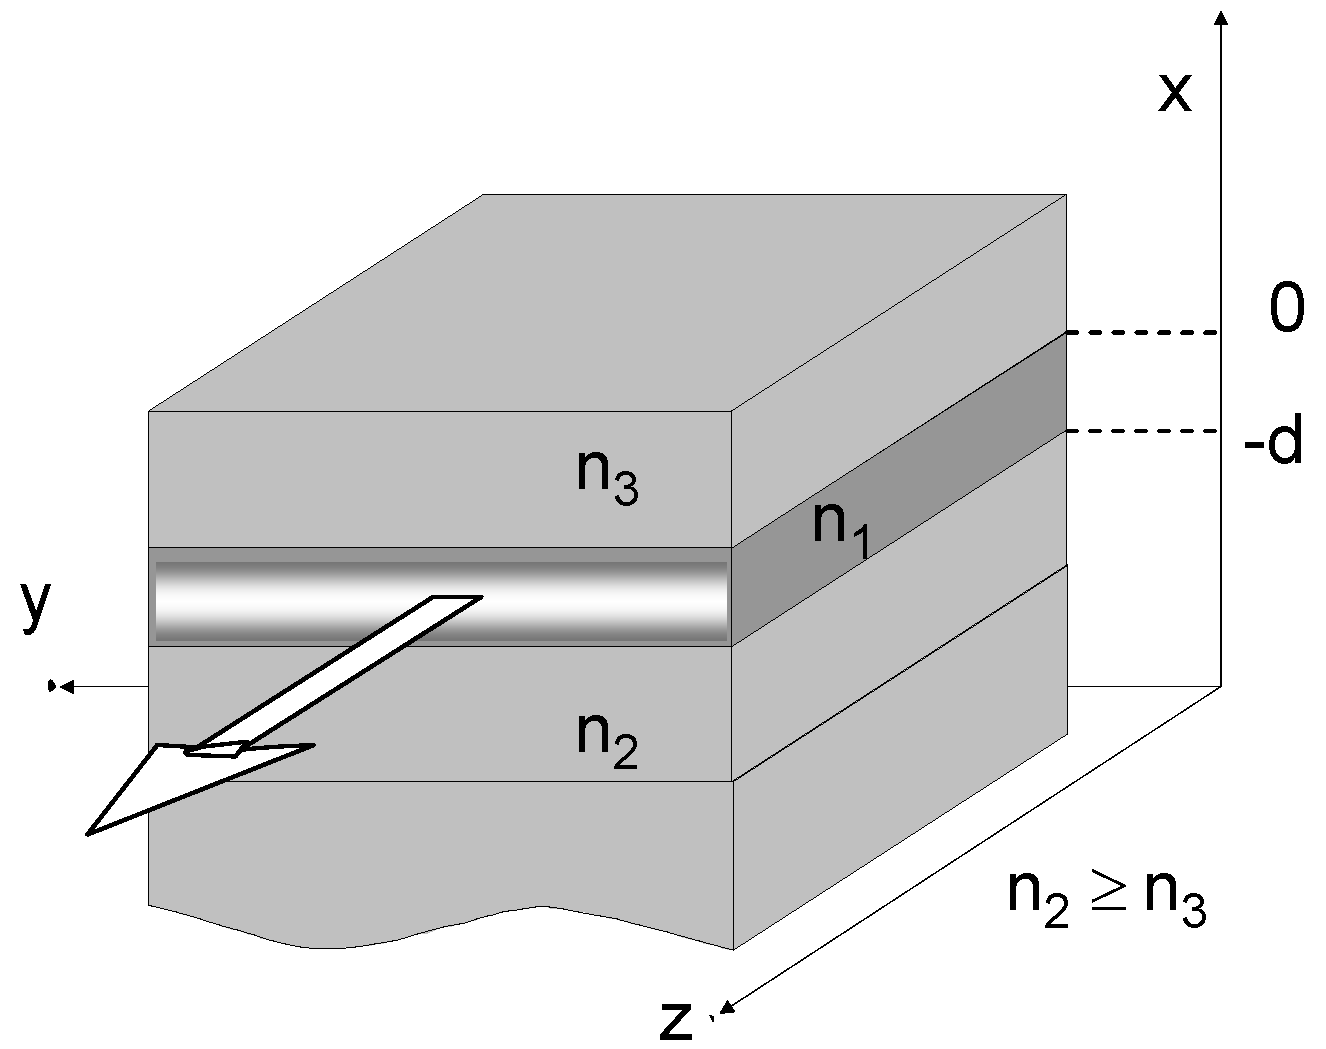
\includegraphics{symmetry/figures/slabwg}
\caption{Slab waveguide.}
\label{fig-slab-wg}
\end{marginfigure}

\begin{cue}
Based on these symmetries, what should be the general form of the eigenmodes of such a structure?
\end{cue}

This means the modes must have the following form:

\begin{equation}
{\mathbf H}_{\mathbf k}({\mathbf r}) = {\mathbf h}(x) e^{-j k_y y} e^{-j k_z z} 
\end{equation} 

Just like we did for the case of inversions, we can classify the modes by their eigenvalue of the symmetry operator, i.e. by their value of ${\mathbf k} = k_y {\mathbf 1}_y + k_z {\mathbf 1}_z$. Although we cannot say anything yet about ${\mathbf h}(x)$ (we need Maxwell for that), we can nevertheless line up the modes in order of increasing frequency. For a given ${\mathbf k}$, we call $n$ the number indicating that mode's place in the line of increasing frequency, so we can identify each mode by its name $({\mathbf k},n)$.
$n$ is called the \textbf{band number}\marginnote{Don't confuse the band number with the refractive index $n$.}. If there is a countable number of modes, $n$ is an integer, but sometimes $n$ may be a continuous variable. 

\begin{marginfigure}
\centering
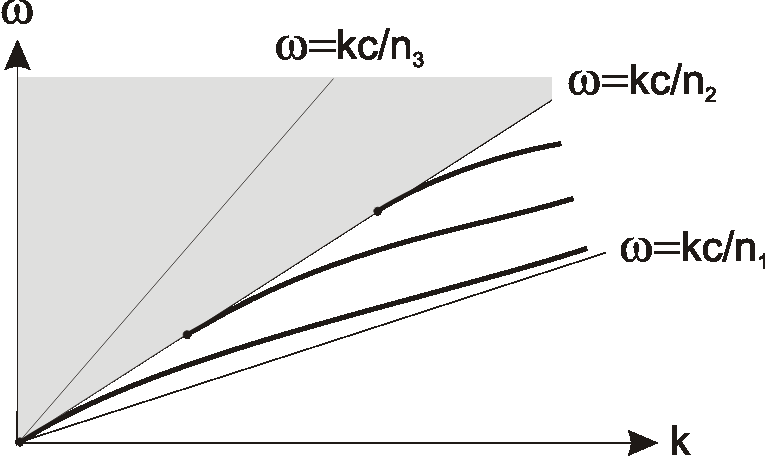
\includegraphics{symmetry/figures/slabdisp}
\caption{Band structure of a slab waveguide.}
\label{fig-slab-disp}
\end{marginfigure}

If for each modal solution that we find, we indicate its wave vector (spatial behaviour) and frequency (temporal behaviour) in a 2D diagram, we notice a continuous evolution if we change wave vector or frequency. What we get is the so-called \textbf{band structure} from Fig.~\ref{fig-slab-disp}. It has been computed by solving Maxwell's equations numerically. The lowest curved line corresponds to the fundamental guided mode of the waveguide (band number $n=0$), the one above that to the first-order mode (band number $n=1$), and so on. The dashed straight lines $\omega=kc/n$ are there to help visualise that the wavevector of a guided mode always lies between the free-space wavevectors of the cladding (with the highest index, in case the upper cladding is different from the lower one) and of the core.

Beware that in some engineering texts this information is presented in a different way. Rather than plotting $\omega$ against $k$, $n_\mathrm{eff}= k \frac {\lambda}{ 2\pi}$ is plotted against $\lambda$, and such a plot is called a \textbf{dispersion relation}.

\begin{cue}
Why do the guided modes in Fig.~\ref{fig-slab-disp} (the lines in the diagram) form a discrete set?
\end{cue}

\begin{marginfigure}
\centering
\includegraphics{symmetry/figures/guided}
\caption{Plane wave picture of a guided mode.}
\label{fig-guided}
\end{marginfigure}

You might recall from basic electromagnetism that a guided mode is basically a plane wave that bounces up and down in the core region, reflecting an infinite number of times at the interfaces with the cladding (Fig.~\ref{fig-guided}). The angle this plane wave makes with the horizontal is related to the propagation constant. Saying that the mode spectrum is discretised, is equivalent to saying that only a specific set of angles of this bouncing plane wave gives rise to an eigenmode, i.e. a field distribution that does not change its shape during propagation. We can only achieve this for special angles where we have a roundtrip phase of $2 \pi$. In other words, this resonance condition discretises the mode spectrum.

With respect to the cladding, some of the light of this bouncing plane wave evanescently leaks out of the core, which explains the exponential decay of the guided modes in the cladding.

Again from basic waveguide theory, you'll recall that for radiation modes on the other hand, the light in the cladding is not an evanescent wave, but rather a standing wave. This also suggests the presence of two plane waves travelling in opposite directions in the cladding.

\begin{cue}
Why do the radiation modes in Fig.~\ref{fig-slab-disp} (the shaded region in the diagram) form a continuous set?
\end{cue}

\begin{marginfigure}
\centering
\includegraphics{symmetry/figures/radiation}
\caption{Plane wave picture of a radiation mode.}
\label{fig-radiation}
\end{marginfigure}

A way to explain this is to first enclose the entire slab waveguide between two metallic mirrors (Fig.~\ref{fig-radiation}), and then study what happens when you move these plates towards infinity, so that you recover the situation of an infinite cladding.

Initially, for a finite distance between the plates, the plates will impose another resonance condition: the plane wave propagating upwards in e.g. the top cladding will be reflected downwards, pass through the core into the bottom cladding, and be reflected upwards again. Again, after one roundtrip, the phase change should be 2 $\pi$ again.

\begin{cue}
What will happen to the separation between the radiation modes in $k$-space as the plates move more and more towards infinity? As an approximation, consider what happens if the space between plates is just filled with air.
\end{cue}

Neglecting the presence of the core, as well as phase shifts upon reflection at the plates, the resonance condition for the phase looks something like $2 d k_x =  2 N \pi$, with $d$ the distance between the plates, $k_x$ the transverse wavevector and $N$ an integer describing the order of the resonance. This shows you that if $d$ goes up, the $k_x$ to realise resonance should go down. In other words, the $k$-vectors get spaced closer together as the distance $d$ increases. In the limit of infinite distance, they will merge together in a single continuum.

A final piece of terminology: the boundary between the discrete guided modes and the continuous radiation modes in the band diagram is called the \textbf{light line}.


\sectionugent{1D discrete translational symmetry and Bloch's theorem}

An important class of systems has \emph{discrete} translational symmetry, i.e. they are not invariant under translations over \emph{any} distance, but only over distances that are a multiple of some fixed step length.

Let's first study systems with such symmetry in one dimension. Higher-dimensional systems will be discussed later.

\begin{marginfigure}
\centering
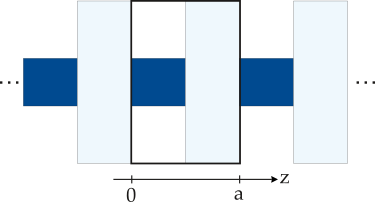
\includegraphics{symmetry/figures/periodic}
\caption{A 1D periodic structure with periodicity $a$ in the $z$--direction.}
\label{fig-1d-periodic}
\end{marginfigure}

Fig.~\ref{fig-1d-periodic} shows a simple structure that is periodic in the $z$--direction, or - to phrase things differently - that has discrete translational symmetry in the $z$--direction. The basic step length is called the \textbf{period} or the \textbf{lattice constant} $a$, and the basic step vector is called the \textbf{primitive lattice vector} ${\mathbf a} = a {\mathbf 1}_z$.

Let's dwell on this concept of lattices a little bit longer, because it will be relevant later as well. A \textbf{lattice} is a collection of vectors which are integer multiples of the primitive latice vectors. There is one primitive lattice vector per dimension, so for our 1D case, its only  ${\mathbf a} = a {\mathbf 1}_z$. Also, it's easy to verify that any integer linear combination of arbitrary lattice vectors will give you another vector belonging to the lattice.

Because of symmetry, $\varepsilon({\mathbf r}) =  \varepsilon({\mathbf r} + {\mathbf a})$, or by repeating this procedure $\varepsilon({\mathbf r}) =  \varepsilon({\mathbf r} + l {\mathbf a})$ with $l$ an integer. The dielectric block that is considered to be repeated over and over is called the \textbf{unit cell} and is highlighted in the square box in Fig.~\ref{fig-1d-periodic}. 


We will now derive an important property of the eigenfunctions of systems with discrete translational symmetry.

Because of the symmetries present, $\Theta$ must commute with all the translation operators over a distance ${\mathbf R} = l a {\mathbf 1}_z$ in the $z$--direction. Again, we will restrict ourselves to the case of scalar fields only varying in the $z$--direction to lighten the notation.

\begin{cue}
Taking a cue from our discussions about continuous translation symmetry, what is the relationship between $H(z + la)$ and $e^{-j k_z la} H(z)$?
\end{cue}

We can follow exactly the same argument that led to Eq.~\ref{eq-bloch-degenerate}, but this time with the set of translations over $la$, to arrive at

\begin{equation}
H(z + la) = e^{-j k_z la} H(z)
\end{equation} 


\begin{marginfigure}[0.5cm]
  % credits: Nobel Prize
  % url: https://www.nobelprize.org/prizes/physics/1952/bloch/biographical/
  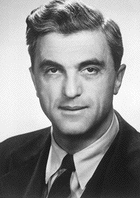
\includegraphics{symmetry/figures/bloch}
  \caption{Felix Bloch (1905-1983)}
\end{marginfigure}

This leads to a first form of Bloch's theorem:

\begin{equation}
\fbox{$\displaystyle  
  H(z + a) = e^{-j k_z a} H(z) \label{eq-bloch-1}
  $}
\end{equation} 

\begin{cue}
Is this mode periodic?
\end{cue}

Note that, although we are working in periodic systems, this mode itself is not periodic, since $H(z + a) \ne H(z)$, but it picks up an extra phase factor.

Eigenfunctions of periodic systems are often called \textbf{Bloch states}.

\begin{cue}
  The equations for waveguide modes (continuous translation symmetry) and Bloch modes (discrete translation symmetry) look suspiciously similar. What is the difference then?
\end{cue}

A crucial difference with the case of continuous translation symmetry is that Eq.~\ref{eq-bloch-1} is only valid for displacements that are an integer multiple of the period, and not for arbitrary displacements, as would be the case for waveguide modes.
 
The number $k_z$ is called the \textbf{wave number} of the Bloch state. Once again, we can use the wave number $k_z$ to classify the modes and draw a band diagram. Compared to the case of continuous translational symmetry however, the wave number has a different interpretation. Rather than saying something about the phase relationship between any two different points on e.g. a slab waveguide, the Bloch wave number only provides information about the phase relationship between points in the structure that are spaced with the same periodicity as the system.


\pagebreak

\sectionugent{The Brillouin zone}

\begin{marginfigure}[-0.0cm]
% credits: AIP Emilio Segre Visual Archives, Leon Brillouin Collection
% url: https://www.researchgate.net/figure/Leon-Brillouin-1889-1969-courtesy-AIP-Emilio-Segre-Visual-Archives-Leon-Brillouin_fig9_270071523
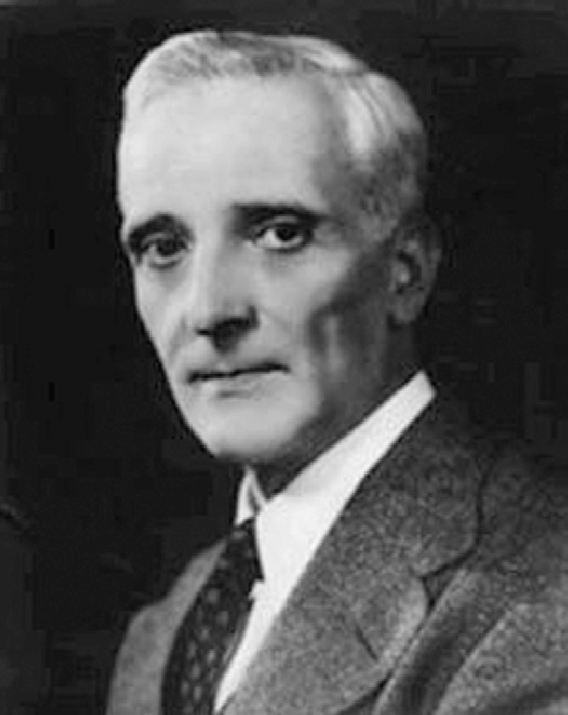
\includegraphics{symmetry/figures/l_brillouin}
\caption{L\'{e}on Brillouin (1889-1969)}
\end{marginfigure}

Looking at Eq.~\ref{eq-bloch-1}, it is clear that the wave number $k_z$ is only defined up to an integer multiple of $2 \pi/a$:

\begin{equation}
e^{-j (k_z + m\frac{2 \pi}{a} ) a} = e^{-j k_z a} e^{-j m 2 \pi} = e^{-j k_z a}
\end{equation} 

Any Bloch state doesn't have just a single wave number $k_z$ at a given frequency, but in fact a whole family of equivalent wave numbers $k_z+m 2 \pi /a$ at that frequency.

This means that we can restrict our band diagram to e.g. the $k_z$--range $[-\pi/a,\pi/a]$. This important region of non--redundant $k_z$--values is called the \textbf{Brillouin zone}.

The band diagram at other $k_z$--values can be constructed by periodic repetition of the Brillouin zone (see Fig~\ref{fig-band-folding}).

\begin{figure}[H]
\centering
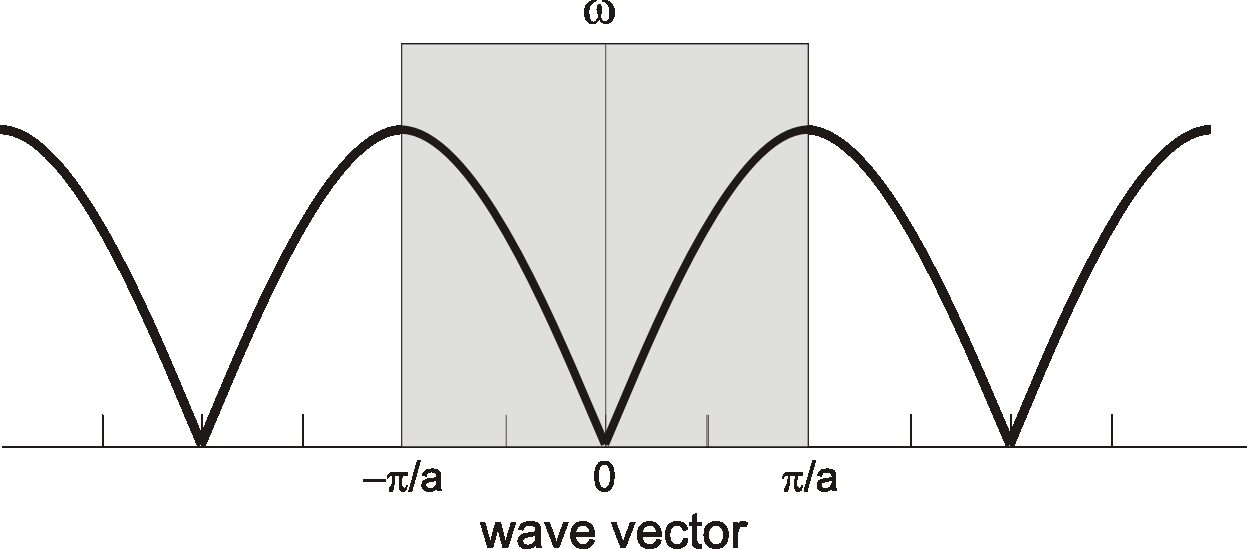
\includegraphics[width=7cm]{symmetry/figures/band_folding}
\caption{Band structure of a periodic system. The Brillouin zone is the hatched region.}
\label{fig-band-folding}
\end{figure}

Ultimately, this periodicity in $k$-space comes from our convention of preferring to using the $k$-vector to label a mode, rather than using the entire phase factor $ e^{-j k_z a}$. 

\pagebreak

\sectionugent{Second form of Bloch's theorem}
\label{week9}

Let's introduce a new function $u$:

\begin{equation}
u(z) = e^{j k_z z} H(z) \label{eq-bloch-u}
\end{equation} 

\begin{cue}
Use Bloch's theorem to show that this function has the same periodicity as the lattice.
\end{cue}

\noindent\marginnote[-2cm]{Sometimes the name of Floquet is also used instead of that of Bloch. The mathematician Floquet first came up with this theory in the context of 1D systems in mechanics, while Bloch later generalised it to 3D in the context of solid state physics.}We start from

\begin{equation}
u(z+la)= e^{j k_z z} e^{j k_z l a} H(z + l a)
\end{equation} 

With Eq.~\ref{eq-bloch-1} this becomes

\begin{equation}
u(z+l a)= e^{j k_z z} e^{j k_z l a} e^{-j k_z l a} H(z) = e^{j k_z z} H(z) = u(z)
\end{equation} 

Rewriting Eq.~\ref{eq-bloch-u}, we can say that the eigenfunctions of a 1D periodic system can be written as

\begin{equation}
\fbox{$\displaystyle  
    H(z) = e^{-j k_z z} u(z) \hspace{.3 cm} \textrm{with} \hspace{.2 cm} u(z+la) = u(z) \label{eq-bloch-state}
$}
\end{equation} 

So, the solution $H(z)$ is a plane wave, as it would be in free space, but modulated by a periodic function because of the periodic lattice. This plane wave modulated by a periodic function is called a \textbf{pseudoperiodic function}.

\begin{cue}
  Given that $u$ is periodic in $z$, write it as a Fourier series involving complex exponentials.
\end{cue} 

Writing $u(z)$ as a Fourier series, we get

\begin{equation}
u(z) =  \sum_{m=-\infty}^{\infty} u_m {e^{-j m \frac{2 \pi}{a} z}}
\end{equation} 

This means that

\begin{equation}
H(z)=  \sum_{m=-\infty}^{\infty} u_m {e^{-j \left( k_z + m \frac{2 \pi}{a} \right) z}}
\end{equation} 

\begin{cue}
Interpret this physically. How does the Brillouin zone come into play again?
\end{cue}

This shows that a Bloch mode is made up of an infinity of plane wave contributions with wave vectors $k_z + m 2 \pi / a$.

It doesn't really matter which of these wavevectors we choose to represent the mode, as we know we can get all the others by looking at wavevectors that are multiples of $2 \pi / a$ away. So, we could conventionally restrict ourselves to wavevectors in the interval $[-\pi/a,\pi/a]$. This is the Brillouin zone argument all over again.


\begin{exer}
% difficulty: trivial
% ugent
% youtube: 6EvNUHZgWLw
Consider a Bloch state $H(z)$ at frequency $\omega$ with wave vector $k$ and described by a certain periodic function $u_k(z)$ as per Eq.~\ref{eq-bloch-state}. The same Bloch state can also be described by another wave vector $k' = k+m 2 \pi / a$. What is the corresponding function $u_{k'}(z)$ for that description?

This illustrates again that it does not matter what 'label' ($k$ or $k'$) we use to stick on our 'box' (the Bloch mode): its 'contents' stay the same.
\end{exer}


\pagebreak

\sectionugent{Example: band gaps in 1D layered stacks}

\begin{marginfigure}
\centering
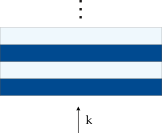
\includegraphics{symmetry/figures/dbr}
\caption{1D periodic stack under normal incidence.}
\label{fig-dbr}
\end{marginfigure}

As a simple example of a periodic system, let's plot the band diagram of a planar multilayered film, consisting of alternating layers of low index and high index materials, each with thickness $a/2$ (see Fig.~\ref{fig-dbr}). This system is periodic in the $z$--direction, and Bloch theory tells us that we only need to consider $k_z$--values in the interval $-\pi / a \le k_z \le \pi / a$. As for $k_x$ and $k_y$, our system has continuous translation symmetry in these directions, so these $k$--components can assume any value. However, let's restrict ourselves to the special case of normal incidence or on--axis propagation, where $k_x=k_y=0$. So, without risk of confusion, we can abbreviate $k_z$ by $k$.

Let's first look at the case of zero index contrast between the materials, so that the medium is completely homogeneous.

\begin{cue}
What do the bands look like in this case? In other words, what is the relationship between $\omega$ and $k$ for solutions to Maxwell's equations in uniform space?
\end{cue}

In such a system, the solutions are plane waves with $\omega = c k / n$, so that band is a straight line in the $(\omega, k)$-diagram, starting from the origin upwards toward the right.

Actually, it turns out there's another solution for negative values of $k$, which is a second straight line $\omega = - c k / n$, starting from the origin and going upwards toward the left.

\begin{cue}
What does this second line correspond to physically?
\end{cue}

This corresponds to waves propagating in the $-z$ direction instead of the $+z$ direction. For structures without reflection, this solution is usually omitted, but we'll see later that for our case, we need to include it.

To make the link to actual periodic structures later on, let's impose an arbitrary artificial periodicity $a$ on this medium.

\begin{cue}
What is the impact of this periodicity on the band diagram?
\end{cue}

This means that, according to Bloch theory, the two lines should repeat themselves starting from the points $k = l 2 \pi / a$. This is illustrated in Fig.~\ref{fig-1d-bands-uniform}.

\begin{figure}[H]
\centering
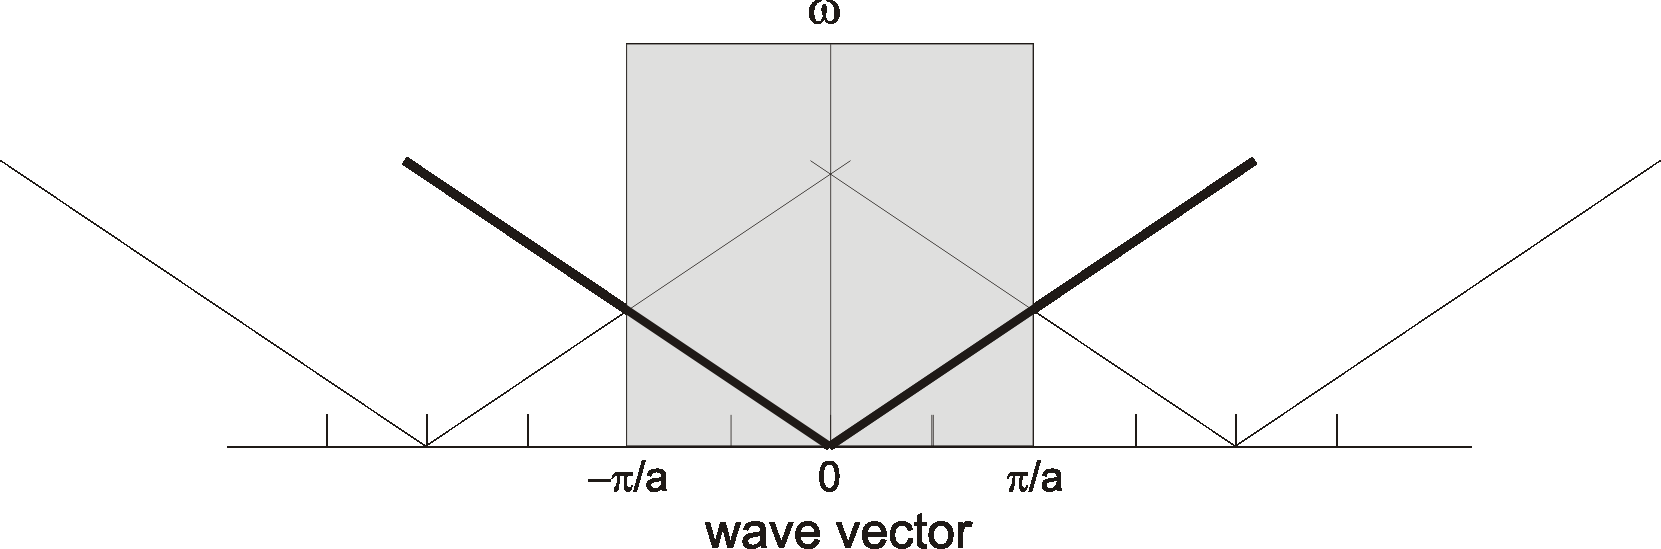
\includegraphics{symmetry/figures/band_folding_uniform}
\caption{Band structures for a uniform medium where we impose an artificial periodicity $a$. The thick lines are the fundamental solutions, the thin lines are copies of this as required by the artificial periodicity.}
\label{fig-1d-bands-uniform}
\end{figure}

When we restrict such a plot to the Brillouin zone, we get the results from the left panel of Fig.~\ref{fig-1d-bands}, with the bands appearing to fold back at the edges of the Brillouin zone. In this figure, we plot the band diagrams $\omega_n(k)$ for three different cases of index contrast between the two layers: zero, low and high. (Note that the wavevector is expressed in units of $\pi /a$, and the frequency in units of $a/c$.) These results have been obtained by numerical calculations.

\begin{figure}[H]
\centering
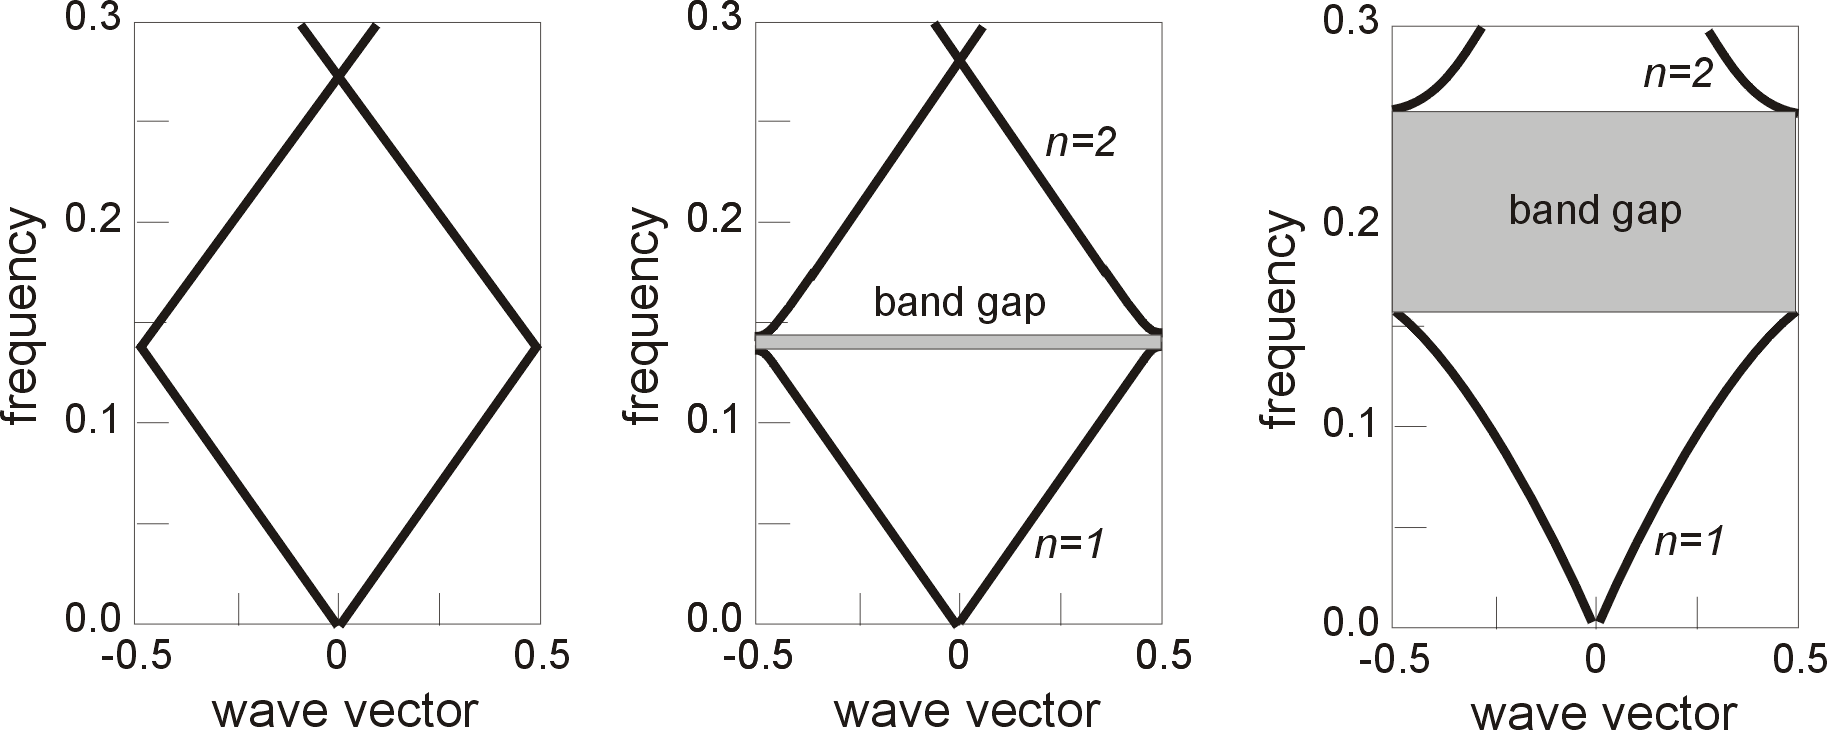
\includegraphics{symmetry/figures/1D_bands}
\caption{Band structures for normal incidence for three different multilayer films where all layers are $a/2$ thick. Left: all layers have $\varepsilon=13$. Middle: layers alternate between $\varepsilon=12$ and $\varepsilon=13$. Right: layers alternate between $\varepsilon=1$ and $\varepsilon=13$}
\label{fig-1d-bands}
\end{figure}

As we increase the index contrast, a curious feature emerges at the edges of the Brillouin zone in Fig.~\ref{fig-1d-bands}. We start to see frequency regions appear where no solutions exist for any $k$. This so--called \textbf{photonic band gap} becomes wider as the index contrast increases.

What is the consequency of having of such a band gap? In this frequency range, there are no allowed propagating states in the system. Suppose we have a semi--infinite periodic system for $z>0$, and a uniform medium for $z<0$.

\begin{cue}
What happens if we excite the semi--infinite periodic system with light coming from the uniform medium below?
\end{cue}

In this situation, the light will find no states to couple to inside the periodic system. Therefore, it has no choice but to return from where it came and be fully reflected. So, inside a band gap, a periodic structure acts as a perfect mirror.

\begin{cue}
Where does such a band gap come from?
\end{cue}

One obvious way of explaining the origin of the band gap, is saying that the reflections from each of the interfaces in the system interfere constructively, such that the system will behave as a perfect reflector and no modes can exist inside it.

Another more convoluted (but educational!) heuristic way of looking at it, is by making use of the heuristics we derived from the variational formulation of Maxwell's equations. Let's look at mode profiles for states immediately above and below the gap. The gap between bands 1 and 2 occurs at the edge of the Brillouin zone, where $k = \pi / a$. If we look at the middle and right diagram of Fig.~\ref{fig-1d-bands}, we see that at the edges, the numerical calculations show us that the bands are horizontal.

\begin{cue}
What are the consequences in terms of wave propagation for such so-called flat bands?
\end{cue}

Since flat bands correspond to $d \omega / dk=0$, this means that the group velocity of the solution is zero. In other words, we are dealing with standing waves here.

\begin{cue}
What is the relationship between the wavelength and the lattice constant in this case?
\end{cue}

At the edge, $k=\pi / a$, so we have standing waves with a wavelength of $\lambda = 2 \pi / k = 2a$, i.e. twice the lattice constant.

For small index contrast, it is logical to assume that the standing waves won't differ too much in shape from those in free space, i.e. they will also be roughly sinusoidal.

\begin{cue}
How can you position a sinusoidal standing wave with wavelength $2a$ with respect to the layer stack, such that you still respect all the symmetries of the system?
\end{cue}

Given that there's inversion symmetry in the middle of each layer, there are only two ways to centre a standing wave of this kind, without violating the symmetry of the system. These are plotted in Fig.~\ref{fig-field-placement}: we can position the peak of the mode either in the low or in the high dielectric region.

\begin{marginfigure}
\centering
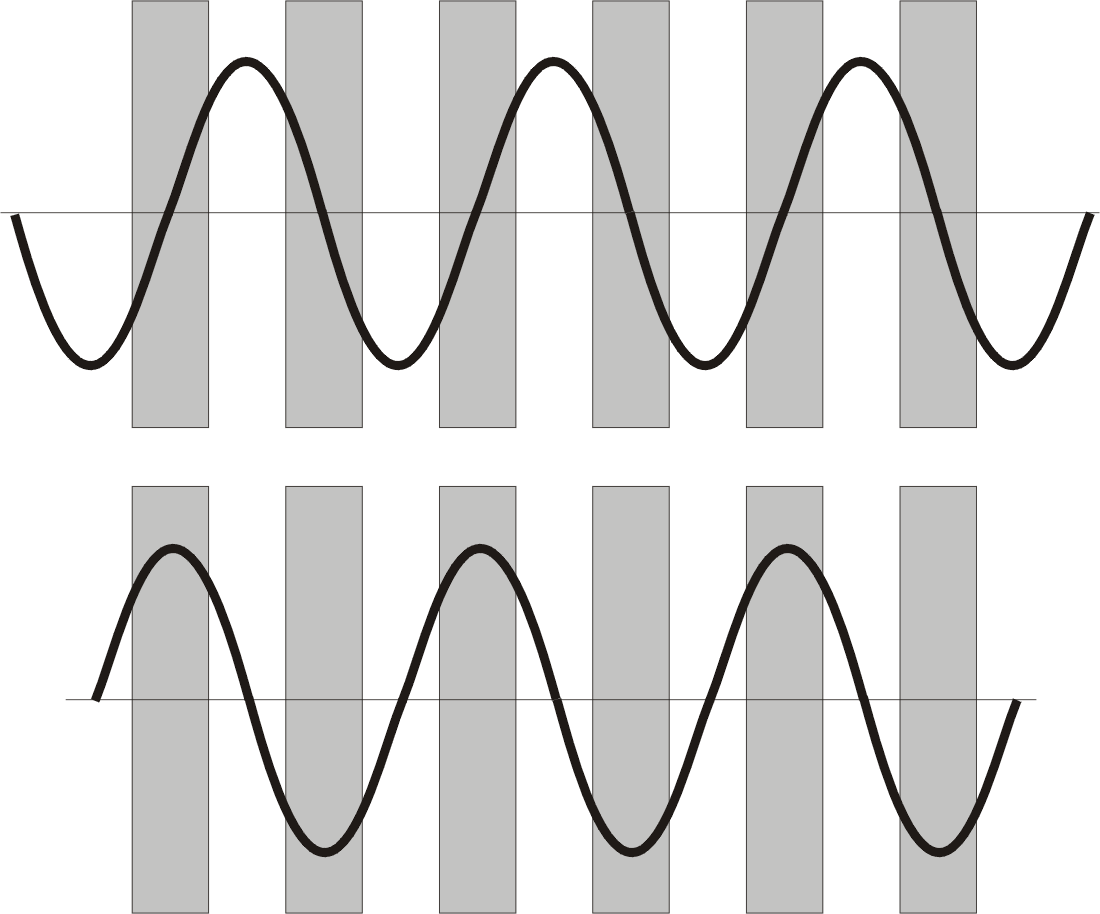
\includegraphics{symmetry/figures/field_placement}
\caption{Two ways to position the field: maximum intensity in the air (top) or in the dielectric (bottom). Note that this is a diagram in real space, i.e. the horizontal axis represents position.}
\label{fig-field-placement}
\end{marginfigure}

\begin{cue}
Recall what we've seen about the frequency of a mode depending on how much it's concentrated in regions with a high refractive index (Section~\ref{sec-sym-var}). What does that mean for the frequencies of the two modes in Fig.~\ref{fig-field-placement}?
\end{cue}

We know from our variational study that a mode that is more concentrated in high dielectric regions will have a lower frequency. So, the two modes from Fig.~\ref{fig-field-placement} will have a different frequency and therefore a gap opens between them.

Since in the low--frequency band the fields are more concentrated in the high dielectric region, this band is usually called the \textbf{dielectric band}. Often, the low dielectric is air, which explains why the upper band is often called the \textbf{air band}.

All of this is completely analogous to semiconductor physics, where the periodicity of the semiconductor crystal gives rise to conduction and valence bands with a forbidden gap in between. In our case, we have artificial periodicity on a larger length scale (comparable to the wavelength of light used), so we call these structures \textbf{photonic crystals}.

In the 1D case, although there is a bandgap for normal incidence for any index contrast, it turns out that this gap will start to close as we move away from normal incidence. This is logical, as in the limiting case of grazing incidence, there is no longer periodicity in the propagation direction.

\pagebreak

\sectionugent{Bloch's theorem in 3D}

The same arguments we used to introduce Bloch's theorem for 1D systems can of course be extended to higher dimensionalities. Following a similar line of reasoning, we can conclude that for any eigenfunction ${\mathbf H}$ of $\Theta$ which describes a periodic system, there exists a vector ${\mathbf k}$ such that for any lattice vector ${\mathbf R}$ the following holds:

\begin{equation}
\fbox{$\displaystyle
{\mathbf H}_{\mathbf k} ({\mathbf r}+ {\mathbf R}) = e^{-j {\mathbf k} \cdot {\mathbf R}} {\mathbf H}_{\mathbf k} ({\mathbf r})
$}
\end{equation} 

Since we label each solution by its wavevector, ${\mathbf k}$ was used a subscript of ${\mathbf H}$.

Completely similar to the 1D argument, we can derive an alternative formulation of Bloch's theorem by saying that any solution ${\mathbf H}_{\mathbf k}$ can be written as

\begin{equation}
\fbox{$\displaystyle
{\mathbf H}_{\mathbf k} ({\mathbf r}) = e^{-j {\mathbf k} \cdot {\mathbf r}} {\mathbf u}_{\mathbf k} ({\mathbf r})
$}
\end{equation} 

The function ${\mathbf u}$ is periodic for all lattice vectors ${\mathbf R}$ of the crystal: ${\mathbf u}_{\mathbf k} ({\mathbf r} + {\mathbf R})  = {\mathbf u}_{\mathbf k} ({\mathbf r})$

Just like in 1D, there is a range of ${\mathbf k}$--values which gives rise to non--redundant solutions which is called the Brillouin zone. However, in higher dimensions it is slightly more complicated to construct this region, so we first spend some time discussing additional tools we need for that.

\pagebreak

\begin{exer}
  % difficulty: normal
  % youtube: qOITP-X6ti4

Using

$$ \nabla \times (\psi {\mathbf A}) = (\nabla \psi) \times {\mathbf A} + \psi (\nabla \times {\mathbf A}) $$
  
show that Bloch modes with wavevector $k$ satisfy the following equation:

$$\Theta_{\mathbf k} {\mathbf u}_{\mathbf k} = \omega^2 \mu {\mathbf u}_{\mathbf k}$$

with

$$\Theta_{\mathbf k} \stackrel{def}{=} (-j {\mathbf k} + \nabla) \times \left [ \frac{1}{\varepsilon({\mathbf r})}(-j{\mathbf k} +\nabla) \times \right ]$$

This formula can be used to build a numerical scheme to calculate Bloch modes: you first fix a value for ${\mathbf k}$ and then solve an eigenvalue problem, where the eigenvalues give the $\omega$--values where Bloch modes appear for this particular ${\mathbf k}$--value.

\end{exer}



\pagebreak

\sectionugent{Reciprocal lattice}

Suppose we have a function $f({\mathbf r})$ that is periodic on a lattice, i.e. $f({\mathbf r} + {\mathbf R}) = f({\mathbf r})$ for all vectors ${\mathbf R}$ that translate the lattice into itself. As we have already seen, these vectors ${\mathbf R}$ are called the \textbf{lattice vectors}.

\begin{cue}
  Write down the continuous Fourier transform of the function $f$, which we can do for any sufficiently well--behaved function. How would you interpret the result physically?
\end{cue}

We get:

\begin{equation}
f({\mathbf r}) = \iiint g({\mathbf k}) e ^ {-j {\mathbf k} \cdot {\mathbf r}} d{\mathbf k}
\end{equation} 

Physically, this means we write $f$ as a sum of plane waves $e ^ {-j {\mathbf k} \cdot {\mathbf r}}$ with wavevectors ${\mathbf k}$ and expansion coefficients $g({\mathbf k})$.


\begin{exer}
  % difficulty: trivial
  % ugent
  % youtube: mwx_fR8CSGo
Make a graphical representation of a plane wave, both in real space and in k-space. What objects live in both spaces? What are the units in each case?
\end{exer}

A Fourier transform like this can be performed on \emph{any} function. But $f$ is not just any function, it is periodic.

\begin{cue}
Exploit the periodicity of $f$ to derive properties of $g$. 
\end{cue}

Periodicity means that

\begin{equation}
f({\mathbf r}) = \iiint g({\mathbf k}) e ^ {-j {\mathbf k} \cdot {\mathbf r}} d{\mathbf k} = f({\mathbf r} + {\mathbf R}) = \iiint g({\mathbf k}) e ^ {-j {\mathbf k} \cdot {\mathbf r}} e ^ {-j {\mathbf k} \cdot {\mathbf R}} d{\mathbf k}
\end{equation} 

From this, we can deduce that

\begin{equation}
g({\mathbf k}) = g({\mathbf k}) e ^ {-j {\mathbf k} \cdot {\mathbf R}}
\end{equation} 

But this is impossible, unless either $g({\mathbf k}) = 0$ or $e ^ {-j {\mathbf k} \cdot {\mathbf R}} = 1$. In other words, the transform $g$ is zero everywhere, except for discrete spikes at ${\mathbf k}$--values where $e ^ {-j {\mathbf k} \cdot {\mathbf R}} = 1$ for all ${\mathbf R}$.

So, what we have just discovered is that if we construct a periodic function using plane waves, we only need to consider those plane waves with wave vectors ${\mathbf k}$ such that $e ^ {-j {\mathbf k} \cdot {\mathbf R}} = 1$ for all lattice vectors ${\mathbf R}$. These ${\mathbf k}$--vectors are called the \textbf{reciprocal lattice vectors} and are usually indicated by ${\mathbf G}$.

\begin{exer}
  % difficulty: trivial
  % ugent
  % youtube: 6eeQw5PlRow
Verify that the  ${\mathbf G}$-vectors form a lattice of their own, i.e. adding two reciprocal lattice vectors yields another reciprocal lattice vector.
\end{exer}

We still need to answer the question of how to build the set of all ${\mathbf G}$--vectors given the set of ${\mathbf R}$--vectors, i.e. find all ${\mathbf G}$ such that ${\mathbf G} \cdot {\mathbf R} = N 2 \pi$ for all ${\mathbf R}$ and for an integer $N$.

Every lattice vector ${\mathbf R}$ can be written as a linear combination of the so--called \textbf{primitive lattice vectors}, which are the smallest vectors pointing from one lattice point to another.

\begin{cue}
  What are the primitive lattice vectors for a cubic lattice?
\end{cue}

For a simple cubic lattice with spacing $a$, all ${\mathbf R}$s are of the form ${\mathbf R} = la {\mathbf 1}_x + ma {\mathbf 1}_y + na {\mathbf 1}_z$, with $(l,m,n)$ integers.

In general, we call the primitive lattice vectors ${\mathbf a}_1$, ${\mathbf a}_2$ and ${\mathbf a}_3$. They don't need to be of unit length.

Since the reciprocal lattice vectors ${\mathbf G}$ also form a lattice, they have a set of primitive vectors ${\mathbf b}_i$ as well, such that ${\mathbf G} = l' {\mathbf b}_1 + m' {\mathbf b}_2 + n' {\mathbf b}_3$.

\begin{cue}
Write a sufficient condition for the requirement that ${\mathbf G} \cdot {\mathbf R} = N 2 \pi$ in terms of these primitive reciprocal lattice vectors.
\end{cue}

Using the primitive reciprocal lattice vectors, this condition can be recast as

\begin{equation}
{\mathbf G} \cdot {\mathbf R} = ( l' {\mathbf b}_1 + m' {\mathbf b}_2 + n' {\mathbf b}_3) \cdot (l {\mathbf a}_1 + m {\mathbf a}_2 + n {\mathbf a}_3)  = N 2 \pi 
\end{equation} 

For all choices of $(l,m,n)$, this must hold for some $N$. That's a lot of different integer combinations here! Let's see if we can come up with an elegant approach to deal with this.


\begin{cue}
Verify that we can satisfy the condition if we happen to find ${\mathbf b}_i$ vectors such that ${\mathbf a}_i \cdot {\mathbf b}_j = 2 \pi \delta_{ij}$, where $\delta_{ij}$ is non--zero only if $i=j$.
\end{cue}

The final question is how to construct these ${\mathbf b}_i$ vectors. We can do this by exploiting the fact that $ {\mathbf x} \cdot ({\mathbf x} \times {\mathbf y}) = 0$ for all vectors ${\mathbf x}$ and ${\mathbf y}$:

\begin{align}
{\mathbf b}_1 =&  \, 2 \pi \frac{{\mathbf a}_2 \times {\mathbf a}_3}{{\mathbf a}_1 \cdot {\mathbf a}_2 \times {\mathbf a}_3} \nonumber \\
  {\mathbf b}_2 =& \, 2 \pi \frac{{\mathbf a}_3 \times {\mathbf a}_1}{{\mathbf a}_1 \cdot {\mathbf a}_2 \times {\mathbf a}_3} \nonumber \\
  {\mathbf b}_3 =& \, 2 \pi \frac{{\mathbf a}_1 \times {\mathbf a}_2}{{\mathbf a}_1 \cdot {\mathbf a}_2 \times {\mathbf a}_3}
\label{eq-recip}
\end{align} 

\begin{cue}
Verify that with this construction, the condition  ${\mathbf a}_i \cdot {\mathbf b}_j = 2 \pi \delta_{ij}$ indeed holds. 
\end{cue}

To summarise, when we build the Fourier transform of a periodic function, we only need to include plane waves with wave vectors that are reciprocal lattice vectors. To construct these reciprocal lattice vectors, we take the primitive lattice vectors and apply Eq.~\ref{eq-recip}.

\begin{exer}
  % difficulty: trivial
  % ugent
  % youtube: gFJlEo0RIqY
In the denominators of Eq.~\ref{eq-recip}, should you evaluate the scalar or the vector product first?
\end{exer}


\pagebreak

\sectionugent{Brillouin zone in 3D}

We already know that for a Bloch mode there exists a vector ${\mathbf k}$ such that

\begin{equation}
{\mathbf H} ({\mathbf r}+ {\mathbf R}) = e^{-j {\mathbf k} \cdot {\mathbf R}} {\mathbf H} ({\mathbf r})
\end{equation} 

\begin{cue}
  Use this formula and what you know about the reciprocal lattice to figure out how to define the Brillouin zone in 3D
\end{cue}

If ${\mathbf k}$ is incremented by a reciprocal lattice vector ${\mathbf G}$, then $e^{-j {\mathbf k} \cdot {\mathbf R}}$ is unchanged by the very definition of reciprocal lattice vector. So, incrementing ${\mathbf k}$ by ${\mathbf G}$ results in the same physical mode.

Therefore, we can restrict our attention to a region in ${\mathbf k}$--space where you cannot get from any point in that region to another in that region by adding a reciprocal lattice vector. This region is the Brillouin zone and consists of all the ${\mathbf k}$--vectors around the origin in reciprocal space that are closer to the origin than to any other neighbouring lattice point in the reciprocal lattice.

These two definitions are equivalent. If a particular ${\mathbf k}$ is closer to a neighbouring lattice point, you can always reach it by staying close to the original point and then translating it by the ${\mathbf G}$ that reaches from one lattice point to the other (Fig.~\ref{fig-bril-bisector}).

\begin{figure}[H]
\centering
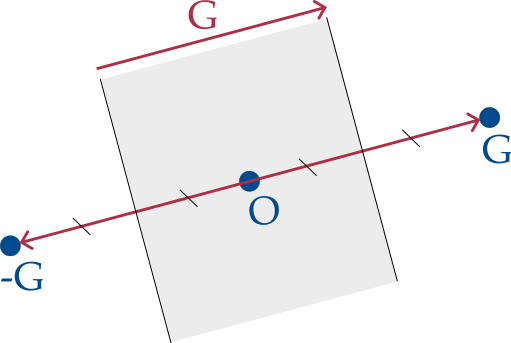
\includegraphics{symmetry/figures/bisector}
\caption{Construction of the Brillouin zone using bisectors of lines joining two lattice points. Any vector ${\mathbf k}'$ that reaches to an arbitrary point on the other side from $A$ can be expressed as the sum of a vector ${\mathbf k}$ on the same side and a lattice vector ${\mathbf G}$.}
\label{fig-bril-bisector}
\end{figure}

To make this more concrete, let's consider the case of a 2D square lattice (Fig.~\ref{fig-bril-square}). Its lattice vectors are ${\mathbf a}_1 = a {\mathbf 1}_x$ and ${\mathbf a}_2 = a {\mathbf 1}_y$.

\begin{cue}
  What is the reciprocal lattice of this square lattice?
\end{cue}

In order to use Eq.~\ref{eq-recip}, we need a third basis vector in the $z$--direction, but for that we can choose one of any length, since the structure is uniform in the $z$--direction. For the reciprocal lattice, we end up with  ${\mathbf b}_1 = 2 \pi / a {\mathbf 1}_x$ and ${\mathbf b}_2 = 2 \pi / a {\mathbf 1}_y$. So, the reciprocal lattice is also a square lattice, but with spacing $2 \pi / a$ instead of $a$.

\begin{cue}
Now construct the Brillouin zone.
\end{cue}

To construct the Brillouin zone, we focus our attention on a particular point (the origin), and draw the lattice vectors that start at the origin. For each of these vectors, we draw the perpendicular bisectors, which divide the lattice into two half--planes (like in Fig.~ \ref{fig-bril-square}), one of which contains the origin. Now repeat this procedure for all lattice vectors near the origin. \noindent\marginnote[-0.7cm]{Depending on the lattice, there could be more vectors to consider than just the primitive lattice vectors and their inverses.} The intersection of all these half--planes forms the Brillouin zone (Fig.~\ref{fig-bril-square}).

\begin{figure}
\centering
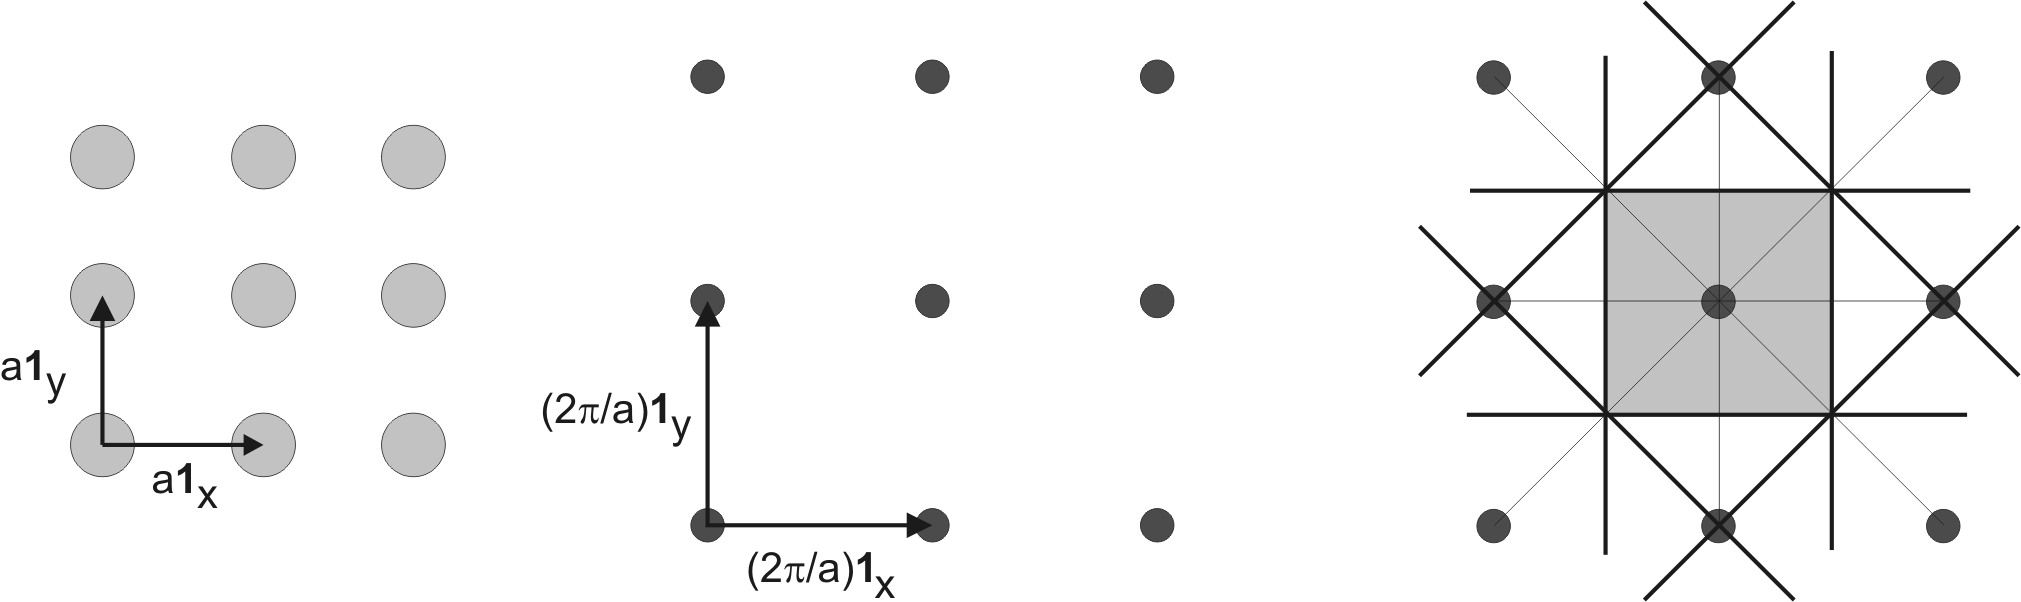
\includegraphics{symmetry/figures/brillouin_square}
\caption{The square lattice. Left: lattice in real space. Middle: lattice in reciprocal space. Right: construction of the Brillouin zone in reciprocal space.}
\label{fig-bril-square}
\end{figure}

\pagebreak
 
\sectionugent{Irreducible Brillouin zone}

Often, a photonic crystal will have additional symmetries. E.g. the square lattice we considered earlier stays invariant for rotations over 90, 180 and 270 degrees. Another symmetry for the square crystal is mirror symmetry about the 45 degrees diagonal. The collection of symmetry operations (rotations, reflections, inversion) for which the crystal is invariant is called the \textbf{point group} of the crystal.

\begin{marginfigure}
\centering
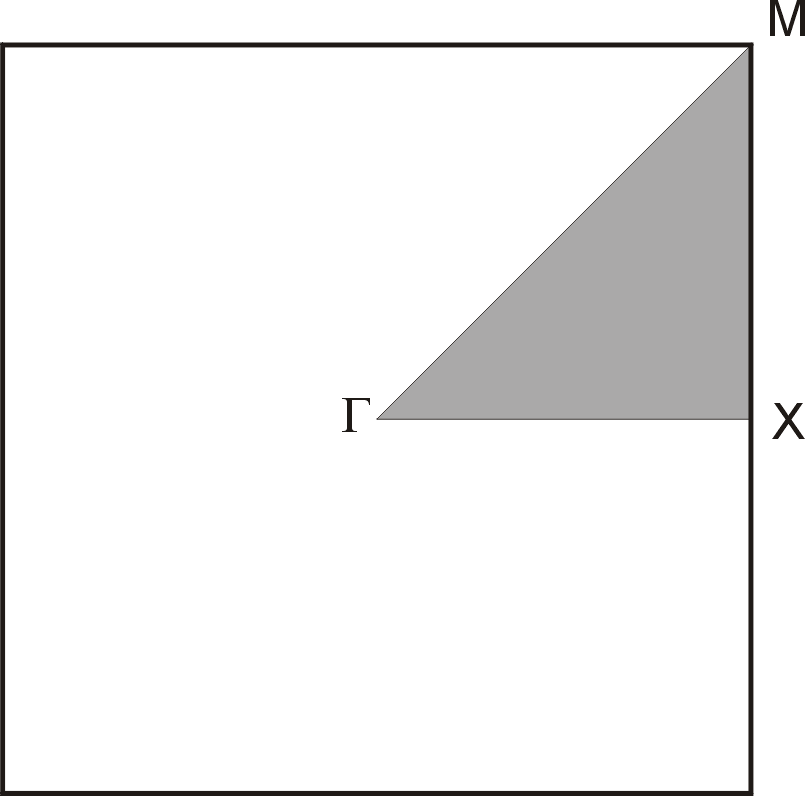
\includegraphics[width=4cm]{symmetry/figures/irred_bril}
\caption{The irreducible Brillouin zone for the square lattice}
\label{fig-irred-bril}
\end{marginfigure}

All of these symmetries mean that there is additional redundancy in the Brillouin zone. The smallest region in the Brillouin zone for which the bands are not related by symmetry is called the \textbf{irreducible Brillouin zone}. As shown in Fig.~\ref{fig-irred-bril}, the irreducible Brillouin zone for the square lattice is a triangular wedge $1/8$ the size of the full Brillouin zone. Also indicated in Fig.~\ref{fig-irred-bril} are some special high--symmetry points of the Brillouin zone. The origin is called the $\Gamma$--point, $X$ is in the direction along the shortest lattice vector and $M$ is in the direction of the diagonal.

Don't get confused: the irreducible Brillouin zone has further symmetries of its own (e.g. drop a line from $X$ perpendicular onto $\Gamma M$), but these are not symmetries of the original crystal, so they can't be used to reduce the Brillouin zone.

Also note that when people talk about a $\Gamma X$ direction, they don't mean just the direction from the origin to the right in Fig.~\ref{fig-irred-bril}, but all the directions that are equivalent because of symmetry.

\begin{exer}
  % difficulty: trivial
  % ugent
  % youtube: KCQaYnUPYXQ
How many $\Gamma M$ and $\Gamma X$ directions are there in a square crystal? Which of these correspond to directions from the origin to nearest neighbours, and which of these to directions from the origin to the second nearest neighbours?
\end{exer}


\begin{exer}
% difficulty: normal
% ugent
% youtube: iyGjzUdby3o
For a triangular (hexagonal) lattice, what are the lattice vectors, reciprocal lattice vectors, Brillouin zone and irreducible Brillouin zone?
\end{exer}

\pagebreak

\sectionugent{Example: 2D square lattice of dielectric rods}

As we have seen, with a 1D periodic structure, we have a band gap for normal incidence regardless of the index contrast. However, if we want to have a gap for oblique incidence too, we will need more--dimensional periodicity: carefully designed 2D structures can have a band gap for all propagation angles in a plane, whereas carefully designed 3D photonic crystals can have a gap for any propagation direction.

We say 'carefully designed structures', because in more dimensions, it is not the case that any periodic structure will automatically give rise to a band gap.

\begin{cue}
Would you prefer a higher or lower index contrast in order to create an omnidirection band gap?
\end{cue}

Obviously, a higher index contrast will help, because it will create stronger reflections for a larger range of incidence angles. Also the nature of the lattice and the shape of the scatterers will play a role. To study the interplay between all these effects, numerical simulations are required.

\begin{marginfigure}[-1.5cm]
\centering
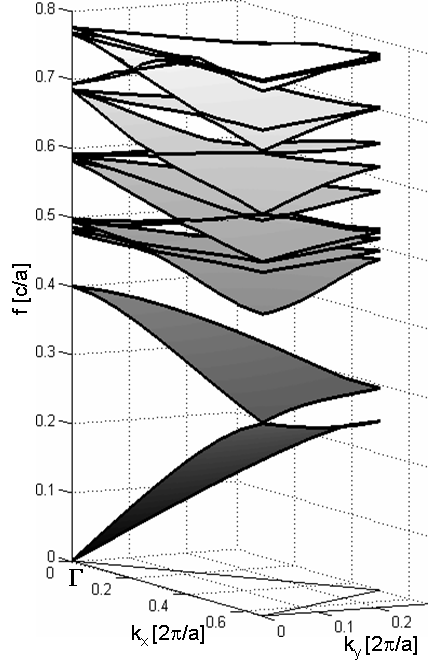
\includegraphics{symmetry/figures/3d_bands}
\caption{Full TM band diagram for a square lattice of dielectric rods, as a set of surfaces in $k$--space.}
\label{fig-bands-rods-3D}
\end{marginfigure}

Remember that in the 1D case, the band diagram plotted the frequency as a function of the 1D wavevector, where the bands were 1D curves. For the 2D case, the frequency is now plotted against the two components of the wavevector, so that we get surfaces instead of curves.

As an example we plot the band structure of a 2D square lattice of dielectric rods in air, for waves propagating in the $xy$--plane. For each ${\mathbf k}$--point in the triangular irreducible Brillouin zone there are a number of bands with increasing frequency. Each band can be plotted as a surface over the irreducible Brillouin zone, as illustrated in Fig.~\ref{fig-bands-rods-3D}.

As such a 3D plot quickly becomes difficult to interpret, people usually only plot the bands along the edges of the irreducible Brillouin zone, as is done in Fig.~\ref{fig-bands-rods}. We can see that there is a bandgap for modes with TM polarisation, but not for TE. In the context of photonic crystals, TM is defined as modes with the ${\mathbf E}$--vector along the rods in the $z$--direction.

\begin{figure}
\centering
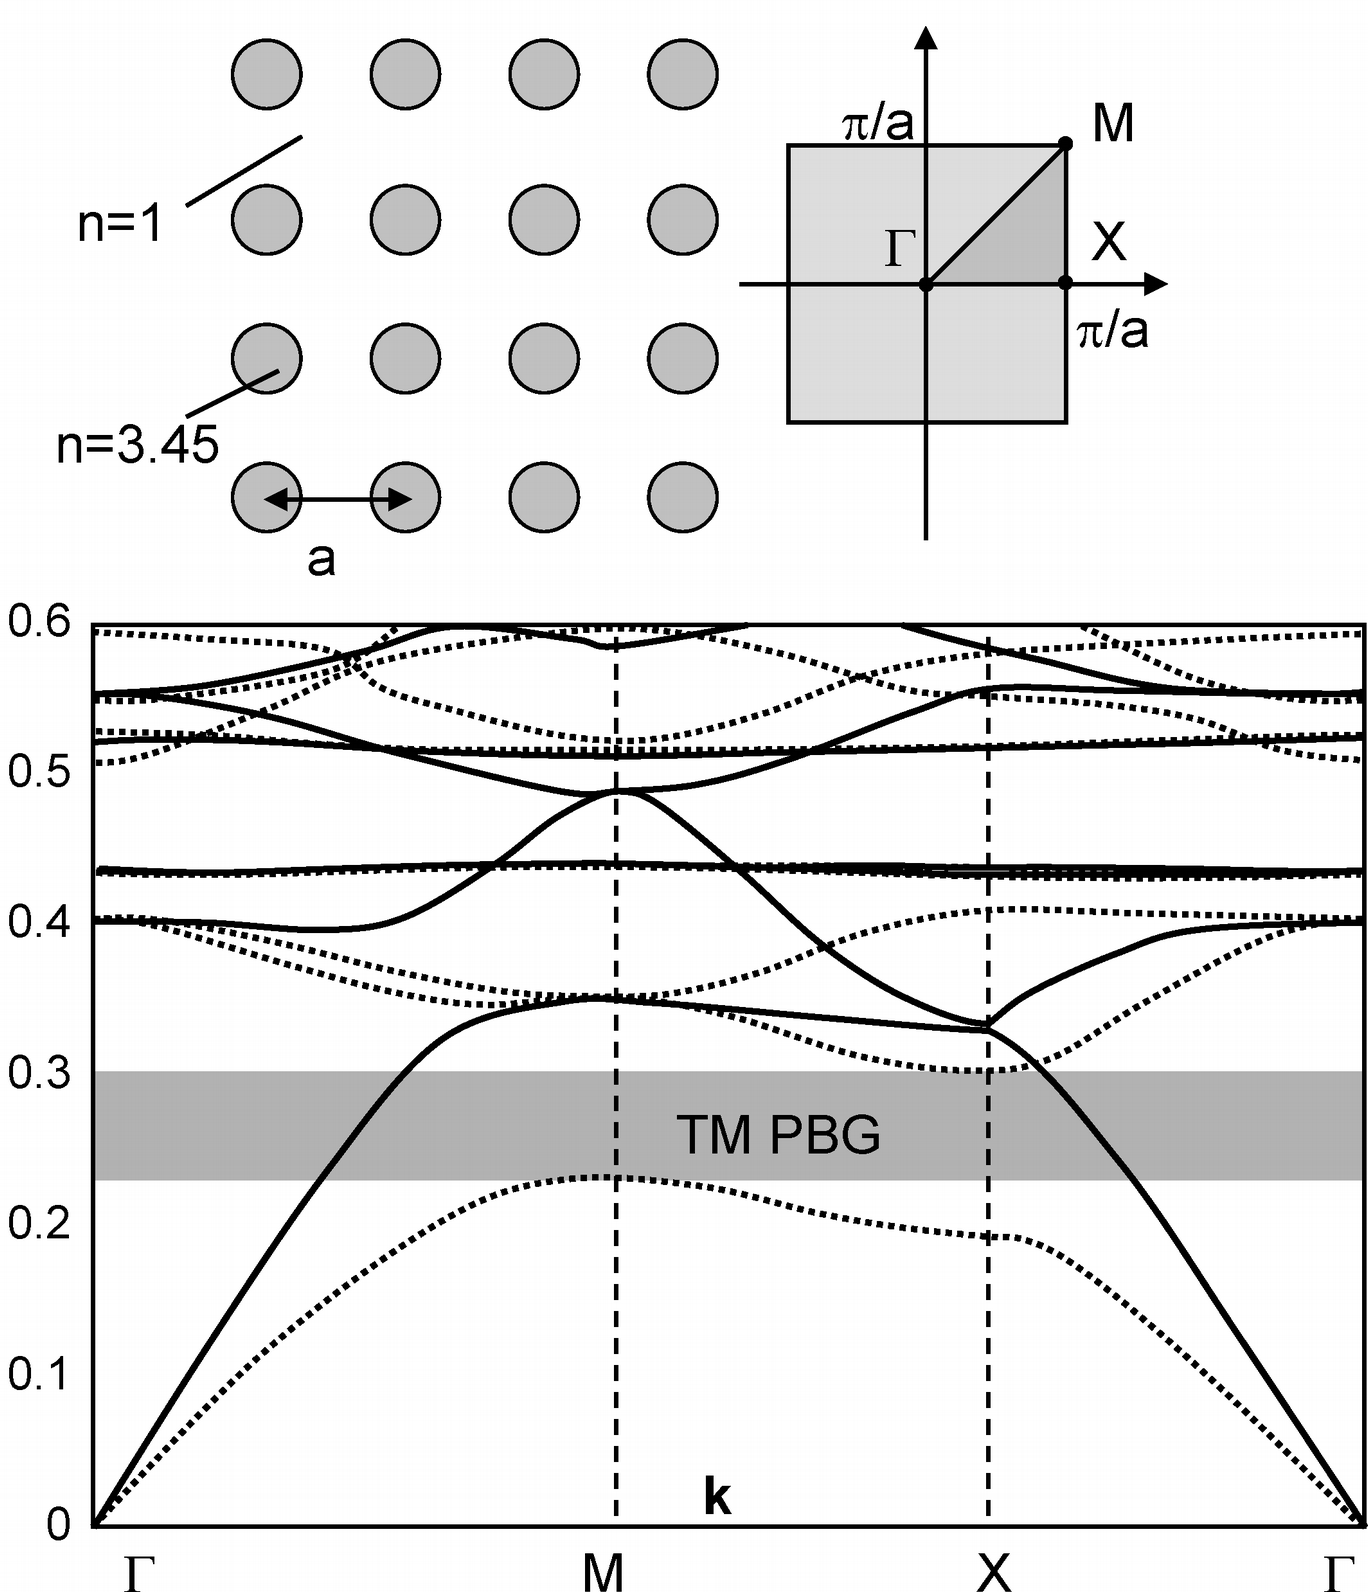
\includegraphics[width=8cm]{symmetry/figures/square_bands}
\caption{Projected band diagram for a square lattice of dielectric rods. Dotted band are TM, full lines are TE polarisation.}
\label{fig-bands-rods}
\end{figure}

\begin{exer}
  % difficulty: normal
  % youtube: _qb090Rsdmc
Based on symmetry arguments, do you think it will be easier to create a 2D omnidirectional bandgap for a square lattice or for a triagular lattice?
\end{exer}

\begin{exer}
  % difficulty: normal
  % youtube: Mr30Uwt45sQ
For a 2D square lattice of dielectric rods, some solutions will be polarised with the electric field parallel to the rods, and some modes will have the electric field perpendicular to the rods. For both situations, calculate the ratio of the electric energy $\epsilon |E|^2$ just inside and just outside the rods. In which case will the electric field be more confined in the rods?
\end{exer}

 
\pagebreak

\section{Time-reversal symmetry}

\begin{exer}
  % difficulty: normal
  % youtube: OknxfFsSkU4
Band diagrams are symmetric around $k=0$, i.e. if there is a mode at frequency $\omega$ with wave vector $k$, there is always a mode at that same frequency with wave vector $-k$. This is true even if the crystal itself does not have inversion symmetry. The mode at $-k$ can be thought of as the backward version of the mode at $k$ and is a consequence of the time reversal symmetry of Maxwell's equations. Make this plausible by taking the following steps:
\begin{itemize}
\item Show that for lossless systems ${\mathbf H}^*$ is also a eigenfunction if ${\mathbf H}$ is an eigenfunction. What is its eigenvalue?
\item Using the definition of phasors, show that if $H_x$ is the phasor corresponding to $ H_{x,0} \cos \left( \omega t + \phi \right)$, then the phasor $H^*_x$ corresponds to the time-reversed signal $ H_{x,0} \cos \left(- \omega t + \phi  \right)$.
\item From the second form of Bloch's theorem, associate ${\mathbf H}^*$ with a Bloch mode at $-k$. What is its corresponding ${\mathbf u}$ function?
\end{itemize}

\end{exer}

\pagebreak

\sectionugent{Applications of photonic crystals}
\label{week10}

Photonic crystals have a lot of similarities compared to electronic crystals, but also some differences. These are summarised in Table~\ref{tab-phot-cryst}.

\begin{table}[h!]
  \begin{center}
    \begin{tabular}{c|c|c} 
      \textbf{Property} & \textbf{Electronic} & \textbf{Photonic}\\
      \hline
      Particle & Electron & Photon \\
      Periodicity & Electron potential & Refractive index \\
      Equation & Schr\"{o}dinger, scalar & Maxwell, vectorial \\
      Bands & Valence, conduction & Dielectric, air \\
      Period & $\sim$ 0.1 nm & $\sim$ 100s of nm \\
      Material & Naturally occurring & Mostly man-made \\
    \end{tabular}
  \end{center}
  \caption{Comparison between electronic crystals and photonic crystals.}
  \label{tab-phot-cryst}
\end{table}


Just as with semiconductors, photonic crystals only become truly useful when defects are introduced in the crystal lattice (Fig.~\ref{fig-defects}).

\begin{figure}[H]
\centering
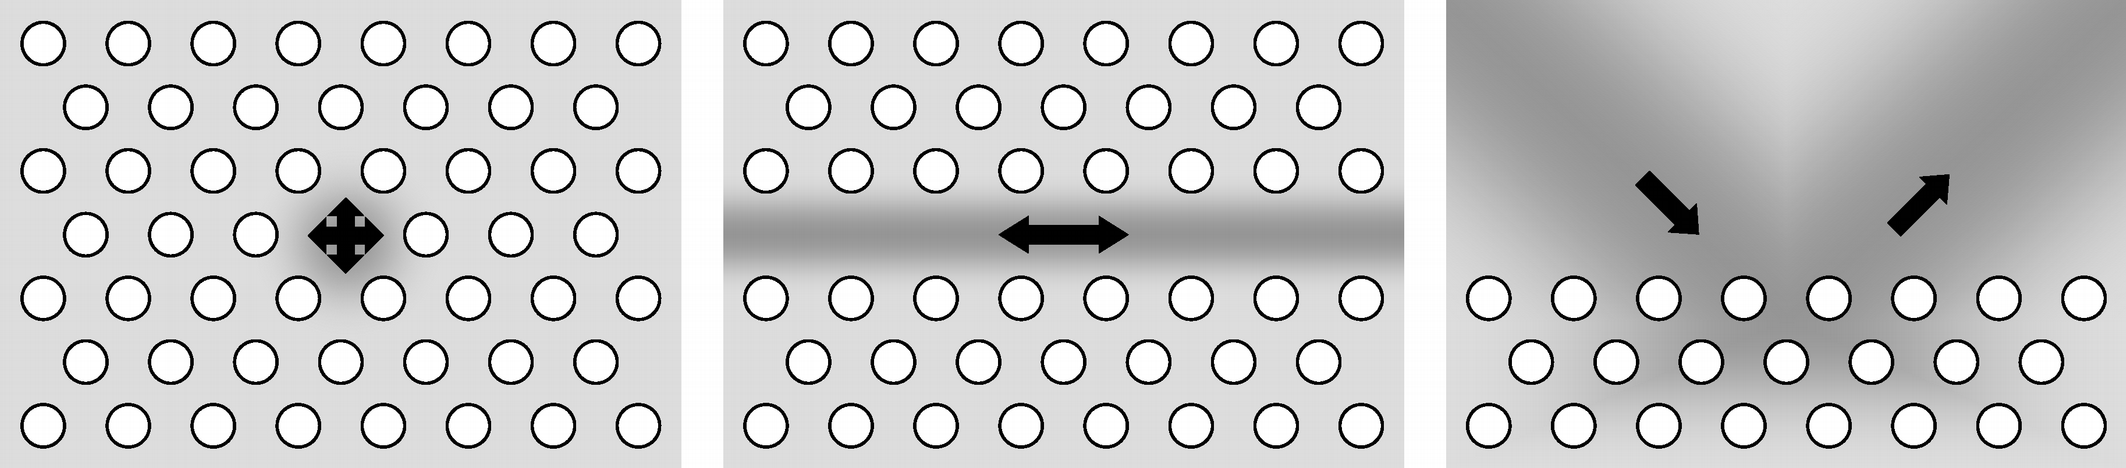
\includegraphics{symmetry/figures/2d_defects}
\caption{Defects in a photonic crystal: a) point defect b) line defect c) surface defect }
\label{fig-defects}
\end{figure}

\begin{cue}
  How do you think light will behave in the presence of these defects?
\end{cue}

When we introduce a point defect in a crystal, we create a small region of space which is surrounded by a photonic crystal which acts as a perfect reflector. So, light has no way to escape from this region and we have created a resonating \emph{cavity}.

Similarly, when we create a line defect, light cannot propagate into the crystal and therefore it has no choice but to follow the line defect. In this way, we have created a \emph{waveguide}.

Finally, we can also create a surface defect, where we just exploit the \emph{mirror} properties of the photonic crystal.

The nice thing about these structures is that they are very small, on the order of the wavelength of the light used. This is why they are often called \emph{nanophotonic} structures. They offer the possibility of miniaturising and integrating a variety of optical components (like e.g. the bends, splitters and filters from Fig.~\ref{fig-components}) onto a single photonic IC.

\begin{figure}
\centering
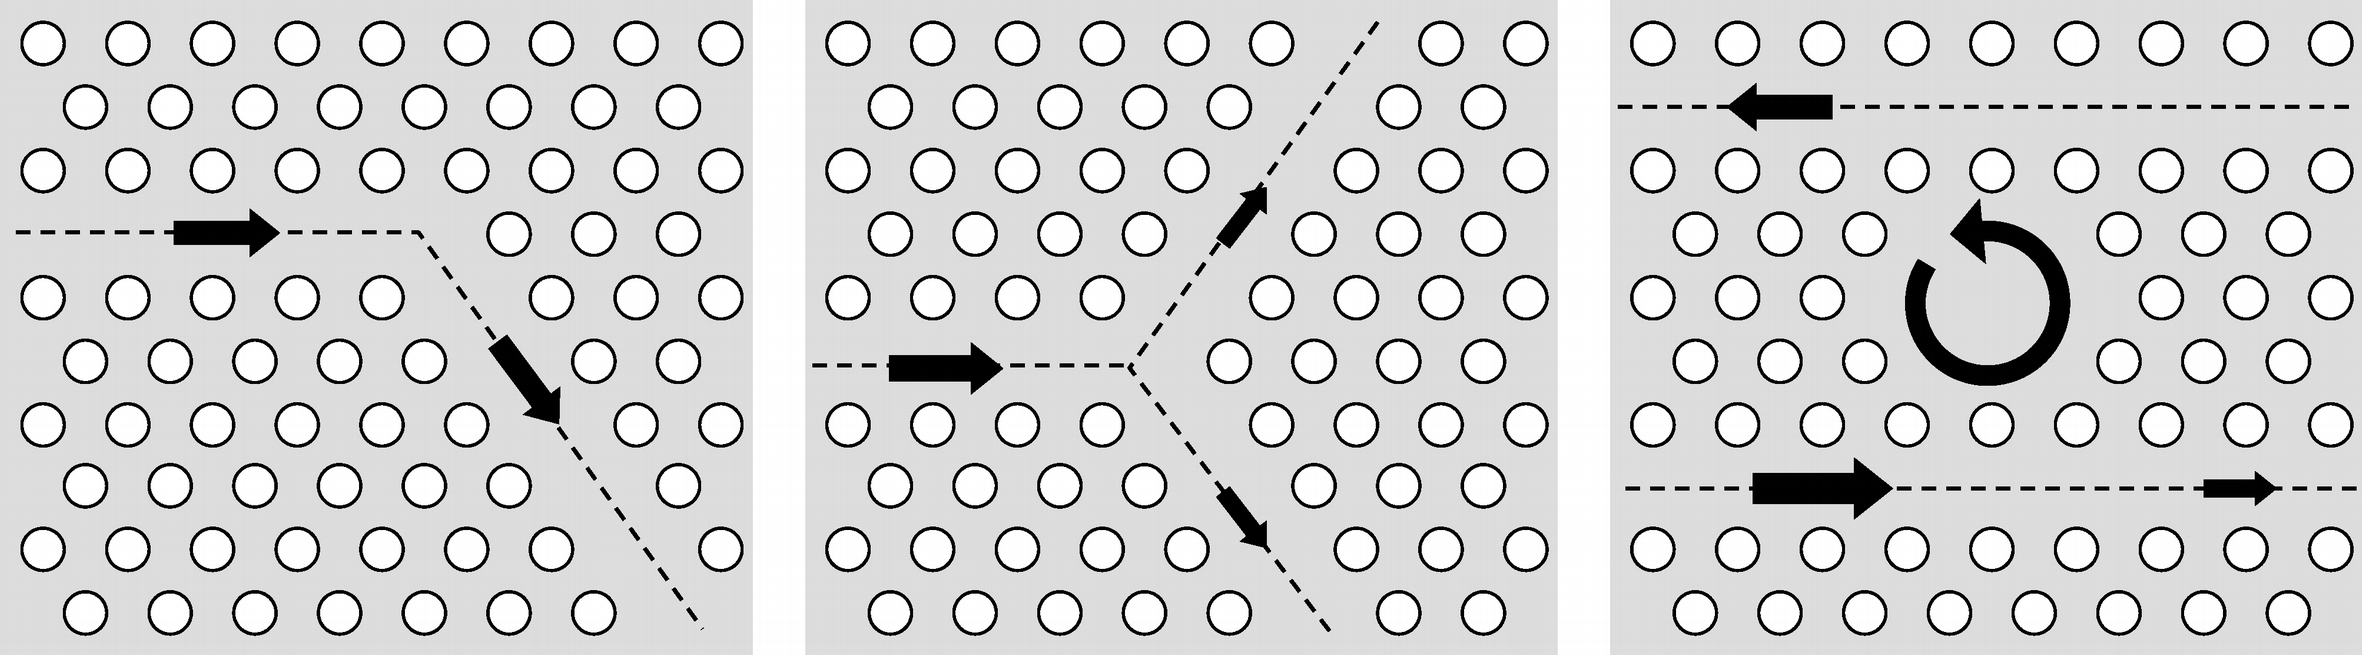
\includegraphics{symmetry/figures/2d_components}
\caption{Example of photonic crystal components: a) bend b) splitter c) resonant filter}
\label{fig-components}
\end{figure}


\section*{Review questions}

\begin{itemize}
\item How do you write the Helmholtz equation as an eigenvalue problem?
\item What are Hermitian operators?
\item What are some properties of Hermitian operators?
\item What physical conclusions can you draw from the variational form of the Helmholtz equation?
\item What is a symmetry?
\item How can you use symmetries to classify modes?
\item What can you say about eigenfunctions in the context of symmetry? 
\item What are degenerate modes?
\item What is a commutator? What does it express in relation to symmetry?
\item What are the similarities and the differences between continuous and discrete translation symmetry?
\item Why do guided modes of a waveguide form a discrete set?  
\item Why do radiation modes of a waveguide form a continuous set?
\item What is the light line?
\item What are two forms of Bloch's theorem?
\item What is a pseudoperiodic function?
\item What is a lattice? Lattice vector? Primitive lattice vector?
\item What is the Brillouin zone?
\item How do you construct the Brillouin zone?  
\item What is the irreducible Brillouin zone?  
\item What is the reciprocal lattice?
\item How do you construct the reciprocal lattice?
\item What are photonic crystals?
\item What do you need to create a photonic band gap?  
\item What are some applications of photonic crystals?  
\end{itemize}





%%% Local Variables:
%%% mode: latex
%%% TeX-master: "../main"
%%% End:
